\documentclass{report}
\usepackage{ugentstyle}
\usepackage{lipsum}
\usepackage{multirow}

\newacronym{ac:hmm}{HMM}{Hidden Markov Model}
\newacronym{ac:hmdm}{HMDM}{Hidden Markov Decision Model}

\newcommand{\regel}[2]{
	\begin{equation*}
		\begin{split}
			& \hbox{\textbf{als} #1} \\
		& 	\hbox{\textbf{dan} #2}
		\end{split}
	\end{equation*}
}


\begin{document}
\maketitle{Kunstmatige intelligentie}
\tableofcontents
\chapter{Kunstmatige intelligentie}


	\begin{itemize}
		\item In deze cursus:
		\begin{itemize}
			\item Genetische algoritmen toegepast op actieve regelbanken.
			\item Bayesiaanse leermethodes toegepast op spraakherkenning.
		\end{itemize}
		\item Twee doelen van kunstmatige intelligentie:
			\begin{itemize}
			\item Het laten overnemen, door machines, van taken waarvoor intelligentie vereist is.
			\item Studie van natuurlijke intelligentie.
			\end{itemize}
		\item Twee vormen om kennis in te brengen in een computersysteem:
			\begin{itemize}
				\item Expliciete kennis (expertsystemen).
				\item Kennis kan zelf verworven worden.
			\end{itemize}
	\end{itemize}
\section{Kunnen machines denken?}
\begin{itemize}
	\item Twee voorbeelden.
	\begin{itemize}
		\item ELIZA:
		\begin{itemize}
			\item Computerprogramma dat zich voordoet als een pyschotherapeut.
			\item Maakt gebruik van simpele vervangingsregels.
			\item Probeert de conversatie zo te sturen zodat de echte persoon het meest moet vertellen.
		\end{itemize} 
		\item Chinese kamer:
		\begin{itemize}
			\item Denkrichting die aantoont dat een entiteit eerst iets moet begrijpen, vooraleer er van intelligentie sprake is. 
			\begin{enumerate}
				\item Iemand die geen Chinees kent wordt in een kamer gebracht.
				\item Door een luik krijgt hij briefjes in het Chinees aangereikt, en de bedoeling is dat hij daar schriftelijk een zinnige antwoord op teruggeeft.
				\item De persoon krijgt handboeken waarin conversieregels staan.
			\end{enumerate}
			\item De proefpersoon volgt mechanisch de regels vanuit het handboek, zodat hij wel intelligent gedrag vertoont, maar de berichten niet begrijpt.
		\end{itemize}
	\end{itemize}
	\item \textbf{Denken is elke vorm van complexe informatieverwerking waarvan de onderliggende mechanismen niet volledig gekend zijn.}
	\item \textbf{Turingtest}:
	\begin{itemize}
		\item Proefpersoon kan contact maken met twee entiteiten: een mens en een machine, maar hij weet niet wie de mens of machine is.
		\item De proefpersoon kan eender welke vragen stellen aan beide entiteiten.
		\item Als de proefpersoon er niet in slaagt om na zijn vragenronde de entiteit aan te duiden die een machine is, dan is de machine geslaagd voor de Turingtest.
	\end{itemize} 
\end{itemize}
\section{Toepassingen van AI en data mining}
\begin{itemize}
	\item \textbf{Classificatie:} 
	\begin{itemize}
		\item Stel een verzameling van $k$ klassen.
		\item Een bepaalde invoer met gelinkt worden aan één van die klassen.
		\item \uline{Harde classificatie:} beperkt aantal duidelijk van elkaar gescheiden klassen. Hier spreekt men ook van patroonherkenning.
		\item \uline{Zachte classificatie:} continue overgang van de klassen. 
	\end{itemize}
	\item Toepassingen:
	\begin{itemize}
		\item Aanbevelingssystemen.
		\item Kwaliteitscontrole.
	\end{itemize}
	\item \uline{Probleemgestuurd}: uitgaande van een probleem een oplossing zoeken.
	\item \uline{Datagestuurd}: vanuit bestaande informatie problemen zoeken die ermee opgelost kunnen worden. Dit wordt ook data mining genoemd. Vaak moet de data eerst gereorganiseerd worden vooraleer de informatie nuttig wordt.
\end{itemize}
\section{Leren}
\begin{itemize}
	\item Moderne AI houdt zich bezig met systemen met een zeer groot aantal aanpasbare parameters. Zulke systemen noemt men \textbf{massief lerende systemen}.
	\item \textbf{Voorbeelden} van massief lerende systemen:
	\begin{itemize}
		\item Neurale netwerken: trachten het biologische denksysteem na te bootsen.
		\item Hidden Markov Model: wordt gebruikt bij de analyse van allerhande sequenties, waarbij de toestand soms onbekend is.
	\end{itemize}
	\item Parameters hebben niet noodzakelijk een betekenis, en is daarom ook onmogelijk om ze met de hand in te voeren. Daarom laat men een systeem leren, met behulp van \textbf{drie methoden}:
	\begin{itemize}
		\item \textbf{Algoritmisch leren}: Er wordt gedemonstreerd hoe een bepaalde actie moet uitgevoerd worden. Het systeem kan hierna deze actie inoefenen door het herhalen van deze instructies. Deze vorm komt goed overeen met het programmeren van een computer.
		\item \textbf{Leren met supervisie}: Hier wordt er geen gebruik gemaakt van een algoritme maar eerder van voorbeelden. Deze voorbeelden worden een leerverzameling genoemd en bevatten inputgegevens die het systeem moet leren herkennen, met de daarbij horende resultaten. Er wordt een verband opgelegd tussen een bepaalde input en output.
		\item \textbf{Leren zonder supervisie}: Dit gebeurt gedeeltelijk algoritmisch aangezien er enige instructies nodig zijn om de machine op gang te krijgen. De machine zal nadien zelf experimenteren wat er gebeurd bij het aanpassen van verschillende parameters. Het leren gebeurt dus niet met voorbeelden, maar uit eigen ervaring. Hier is er dan ook geen verband tussen het resultaat en de verschillende deeltaken, maar er is wel een algemeen idee wat er aangeleerd moet worden.
	\end{itemize}
\end{itemize}
\section{Classificatie}
\begin{itemize}
	\item Classificatie is het mappen van een bepaalde input op een klasse.
	\item We spreken van een \textbf{item} dat we moeten klasseren.
	\item Dit item wordt gekarakteriseerd door een aantal \textbf{meetwaarden}.
	\item \underline{Twee soorten meetwaarden}:
	\begin{itemize}
		\item Sommige metingen kunnen een groot aantal waarden opleveren die voorgesteld kunnen worden als een getal.
		\item Andere metingen hebben maar een beperkt aantal waarden, zoals de indeling van categorieën. 
		\begin{itemize}
			\item Deze kunnen omgezet worden zodat ze antwoorden zijn op ja-nee vragen, zodat ze geconverteerd kunnen worden naar 0 of 1.
			\good Nu zijn alle meetwaarden getallen.	
		\end{itemize}
	\end{itemize}
	\item Aangezien dat alle meetwaarden getallen zijn $\rightarrow$ standaardvorm: de computer heeft een aantal klassen en moet een getallenrij die de meetwaarden voor een bepaal item bevat toewijzen aan één van de klassen.
	\item Hoe worden de getallenrijen weergegeven? Een aantal notaties:
	\begin{itemize}
		\item De $n$-dimensionale Euclidische ruimte is de de verzameling vectoren met $n$ reële coördinaten.
		\item Zo een vector wordt voorgesteld door een vette letter: $\textbf{v} = (v_1, ..., v_n)$.
		\item Soms vanaf 0 beginnen, zodat we $n+1$-dimensionale vectoren hebben: $\textbf{v} = (v_0, v_1, ..., v_n)$. De waarde $v_0$ krijgt een speciale betekenis.
		\item Reeële getallen die niet deel uitmaken van een vector worden weergegeven met hoofdletters: A, B, ...
		\item De nulvector: 0 = (0, ..., 0).
		\item Het inproduct:
		$$\textbf{v}\cdot\textbf{u} = \sum_{i}^{n}v_iu_i$$
		Het inproduct is lineair:
		\begin{itemize}
			\item $(A\textbf{v})\cdot \textbf{u} = A(\textbf{v}\cdot\textbf{u})$
			\item $(\textbf{u} + \textbf{v})\cdot\textbf{x} = \textbf{u} \cdot \textbf{x} + \textbf{v} \cdot \textbf{x}$
		\end{itemize}

		
		Het kan ook gedefinieerd worden als 
		$$\textbf{v}\cdot\textbf{u} = || \textbf{v} ||\;|| \textbf{u} || \cos\theta$$
		met $\theta$ de hoek tussen vector $\textbf{v}$ en $\textbf{u}$.
		
		Als $\textbf{v}$ en $\textbf{u}$ orthogonaal zijn $(\theta = \pi/2)$, dan is het inwendig product:
		$$\textbf{v}\cdot\textbf{u} = 0$$
		
		Als $\theta = 0$, dan 
		$$\textbf{v}\cdot\textbf{u} = || \textbf{v} ||\; ||\textbf{u} ||$$
		
		Hieruit volgt 
		$$\textbf{u} \cdot \textbf{u} = ||\textbf{u}||^2$$
		\item $d(u,v) = ||\textbf{u} -\textbf{v}||$ is de lengte van de kortste weg van \textbf{u} naar \textbf{v}.
		 Hieruit volgt:
		$$||\textbf{u} + \textbf{v}|| \leq ||\textbf{u}||+||\textbf{v}||$$
		 Het kwadraat van beide kanten geeft:
		 $$\textbf{u} \cdot \textbf{v} \leq ||\textbf{u}||\;||\textbf{v}||$$
		 Aangezien dat 
		 $$\cos(\textbf{u}, \textbf{v}) = \frac{\textbf{u} \cdot \textbf{v}}{||\textbf{u} ||\;|| \textbf{v} ||}$$
		 kan dit omgevormd worden tot de volgende ongelijkheid:
		 $$-1 \leq \frac{\textbf{u} \cdot \textbf{v}}{||\textbf{u} ||\;|| \textbf{v} ||} \leq 1$$
		 \item De afstand en de cosinus geven vaak een goede indruk in hoeverre twee vectoren op elkaar lijken. De cosinus geeft een goede maat voor de afstand tussen twee genormaliseerde vectoren:
		 $$d\bigg(\frac{\textbf{u}}{||\textbf{u}||}, \frac{\textbf{v}}{||\textbf{v}||}\bigg)^2 = 2 - 2\cos(\textbf{u}, \textbf{v})$$
	\end{itemize}
\end{itemize}

\section{Informatie en beslissingsbomen}
\subsection{Informatie-inhoud}
	\begin{itemize}
		\item Een bericht is enkel nuttig indien ontvanger een betekenis kan geven aan het bericht. De belangrijke elementen voor de informatie-inhoud is dus het bericht zelf en de kennis van de ontvanger.
		\item Met de kennis kan aan elk mogelijk bericht $B$ een waarschijnlijkheid $P(B)$ toekennen. De informatie-inhoud wordt dan gedefinieerd door
		$$-\log_2(P(B))\; \hbox{bits}$$ 
		Voor $P(B) = 1$ is de informatie-inhoud 0 bits, wat logisch is aangezien de ontvanger niets heeft bijgeleerd van dit bericht.
		\alert De informatie-inhoud van een bericht is niet altijd een geheel getal.
		\alert De informatie-inhoud is nooit negatief.
		\item \underline{Voorbeeld:} Stel dat een byte verwacht wordt, maar er is geen idee welke byte. Elke byte is even waarschijnlijk met kans $1/256$. De informatie-inhoud van de byte die dan binnenkomt is $-\log_2 (1/256)\;\hbox{bits} = 8 \;\hbox{bits}$.
		\item \underline{Voorbeeld:} Stel een alfabet van 4 letters: A, C, G en T. De waarschijnlijkheid dat ze voorkomen wordt weergegeven in tabel \ref{table:example_entropy}.
		\begin{table}[h]
			\centering
			\begin{tabular}{l | r}
				A & 70,71 \% \\
				C & 12,50 \% \\
				G &  8,39 \% \\
				T & 8,39 \% \\
			\end{tabular}
			\caption{De waarschijnlijkheden voor de letters A, C, G en T.}
			\label{table:example_entropy}
		\end{table}
	
		Als de ontvanger dit weet dan wordt de informatie-inhoud voor elke letter:
		
		\begin{equation*}
			\begin{split}
				A: -\log_2(0,7071) & = 0,5 \\
				C: -\log_2(0,1250) & = 3,0 \\
				G: -\log_2(0,0839) & = 3,575\\
				T: -\log_2(0,0839) & = 3,575
			\end{split}
		\end{equation*}
	\end{itemize}
\subsection{Beslissingsboom}
	\begin{itemize}
		\item Elke knoop dat geen blad is bevat een vraag met een beperkt mogelijk aantal antwoorden.
		\item Elk mogelijk antwoord verwijst naar een kind van de knoop.
		\item Een item klasseren is een pad vanuit de wortel naar een blad, waarin de klasse staat.
		\item Hoeveel informatie kan een beslissingsboom geven?
		\begin{itemize}
			\item Stel $k$ klassen $K_1, K_2, ... K_k$.
			\item Stel een verzameling $S$ van items waarbij:
			\begin{itemize}
				\item $A(S, i)$ het aantal elementen horend bij $K_i$ is in de verzameling en,
				\item $|S| = \sum_{i = 1}^k A(S,i)$ het totaal aantal element is van $S$.
			\end{itemize} 
			\item De informatie geleverd door een correcte klassering van alle element is dan:
			
			 {\color{OliveGreen}(groene formules moeten niet van buiten geleerd worden. Ze worden gegeven bij de examenvraag)}
			{\color{OliveGreen}
			\begin{equation*}
				\begin{split}
					E(S) & = \sum_{i = 1}^{k} A(S, i) \bigg(-log_2 \bigg( \frac{A(S, i)}{|S|}\bigg) \bigg) \\
					     & = |S|log_2(|S|) +  \sum_{i = 1}^{k} A(S, i)(-log_2(A(S, i)))
				\end{split}
			\end{equation*}
			}
			Hierbij is $\frac{A(S, i)}{|S|}$ de kans om een item te hebben in klasse $i$.
		\end{itemize}
		\end{itemize}
		\begin{itemize}
			\item Het \textbf{Iterative Dichotomiser 3 (ID3)} is een \underline{inhalig} algoritme dat een beslissingsboom opstelt vanuit een bepaalde dataset.
			\begin{itemize}
				\item De wortel bevat de vraag die het meeste informatie oplevert.
				\item Als het $j$-de attribuut de leerverzameling $L$ in de deelverzamelingen $L_{j,1}, L_{j,2},...,L_{j,n}$ opdeelt, dan is de informatie geleverd door dit attribuut gelijk aan:
				$$I(j) = E(L) - \sum_{m = 1}^{n_j} E(L_{j, m})$$
				Hierbij is $m$ de verschillende waarden dat dit attribuut kan aannemen.
				\item Het attribuut wordt gekozen waarvoor $I(j)$ maximaal wordt.
				\alert Als $I(j) = 0$, dan behoren ofwel alle items tot dezelfde klasse, ofwel kan er op basis van het attribuut geen klassering gemaakt worden.
				\item Na de constructie van de wortel moeten nog $n_j$ deelbomen geconstrueerd worden.
				\item \underline{Voorbeeld:}
				\begin{itemize}
					\item Veronderstel volgende informatie (tabel \ref{table:example}):
					\begin{table}[ht]
						\centering
						\begin{tabular}{| c c c c | r |}
							\hline
							Beroepscategorie & Jonger dan 20? & Fraudeur? & risico? & frequentie \\
							\hline
							A & ja & ja & veilig & 10 \\
							A & ja & nee & riskant & 11 \\
							A & nee & ja & riskant & 18 \\
							A & nee & nee & veilig & 100 \\
							\hline
							B & ja & ja & veilig & 180 \\
							B & ja & nee & riskant & 8 \\
							B & nee & ja & riskant & 1 \\
							B & nee & nee & veilig & 90 \\
							\hline
						 	C & ja & ja & veilig & 50 \\
							C & ja & nee & riskant & 5 \\
							C & nee & ja & riskant & 5 \\
							C & nee & nee & veilig & 50 \\	
							\hline		
							\multicolumn{2}{|r}{}&\multicolumn{2}{l}{Totaal veilig:}	 & 480	 \\
							\multicolumn{2}{|r}{}&\multicolumn{2}{l}{Totaal riskant:}	 & 48	 \\
							\multicolumn{2}{|r}{}&\multicolumn{2}{l}{Algemeen totaal:}	 & 528	\\
							\hline		
						\end{tabular}
						\caption{}
						\label{table:example}
					\end{table}
					\item Voor elk attribuut kan de resulterende verdeling afgeleidt worden (tabel \ref{table:resulterende_verdeling}):
					\begin{table}[ht]
						\centering
						\begin{tabular}{|l | l |rr|}
							\hline	
							Attribuut & waarde & \# veilig & \# riskant \\
							\hline	
							\multirow{3}{*}{(1) Beroepscategorie} & A & 110 & 29 \\
							& B & 270 & 9  \\
							& C & 100 & 10 \\
							\hline	
							\multirow{2}{*}{(2) Jonger dan 20?} & ja & 240 & 24 \\
							& nee & 240 & 24 \\
							\hline	
							\multirow{2}{*}{(3) Fraudeur?} & ja & 240 & 24 \\
							& nee & 240 & 24 \\
							\hline			
						\end{tabular}
						\caption{}
						\label{table:resulterende_verdeling}
					\end{table}
					\item Voor elk attribuut kan nu $I(j)$ berekent worden, hier uitgewerkt voor de beroepscategorie:	
					\begin{equation*}
						\begin{split}
							I(1) & = E(L) - \sum_{m = 1}^{n_1} E(L_{1, m})\\ 
							     & = E(L) - (E(L_A) + E(L_B) + E(L_C)) \\	
							     & \hbox{met} \\
							     E(L) & = 480(-\log_2(480/528)) + 48(-log_2(48/528)) \\
							          & = 232.054 \\
							     E(L_A) & = 110(-log_2(110/139)) + 29(-log_2(29/139)) \\
							            & = 102.702 \\
							     E(L_B) & = 270(-log_2(270/279)) + 9(-log_2(9/279))\\
							     		&  = 57.3603 \\
							     E(L_C) & = 100(-log_2(100/110)) + 10(-log_2(10/110)) \\
									     & = 48.3447\\ 
									     & \hbox{zodat} \\
							I(1) & =  E(L) - (E(L_A) + E(L_B) + E(L_C)) \\
							 	 & = 232.054 - 102.702 - 57.3603 - 48.3447 = 23.647							         	     
						\end{split}
					\end{equation*}
					\item Voor $I(2)$ en $I(3)$ bedragen beide uitkomsten $0$, aangezien er op basis van die attributen geen informatie kan achterhaald worden. Dit is logisch aangezien de verhouding veilige/risicohoudende klanten voor zowel leeftijd als fraudeur 10:1 is.
					\item Als wortel van de beslissingsboom wordt als criterium de beroepscategorie genomen.
					\item Voor zowel $L_A$, $L_B$ en $L_C$ moet apart dezelfde methode uitgevoerd worden. Het kan perfect mogelijk zijn dat op het tweede niveau bij keuze $A$ eerst wordt gecheckt op fraude, maar bij keuze $C$ eerst op leeftijd. 
					\alert Bij $L_C$ levert geen enkel van de twee attributen informatie op, zodat er random moet gekozen worden:
					\begin{table}[ht]
						\centering
						\begin{tabular}{|l | l |rr|}
							\hline	
							Attribuut & waarde & \# veilig & \# riskant \\
							\hline	
							\multirow{2}{*}{(2) Jonger dan 20?} & ja & 50 & 5 \\
							& nee & 50 & 5 \\
							\hline	
							\multirow{2}{*}{(3) Fraudeur?} & ja & 50 & 5 \\
							& nee & 50 & 5 \\
							\hline			
						\end{tabular}
					\end{table}
					\item \underline{Verfijningen:}
					\begin{itemize}
						\item Invoeren van een drempelwaarde voor de informatiewinst. Als deze te klein is wordt er niet meer opgesplitst. Een blad kan dan meerdere klassen bevatten, elk met een waarschijnlijkheid.
						\item Voor elk mogelijk paar van attributen de informatiewinst berekenen en, als deze te groot is, knopen maken met twee attributen.
						\item Bij effectieve getallen kan ook een drempelwaarde ingevoerd worden. Alle items met een waarde kleiner dan deze drempelwaarde gaan naar links, de andere naar rechts. Voor elke mogelijke drempelwaarde moet de informatiewinst berekend worden.
					\end{itemize}
				\end{itemize}
			\end{itemize}
			
		\end{itemize}

\section{Klasseren zonder leren}
\begin{itemize}
	\item Klassen worden niet vooraf gegeven.
	\alert Geen leerverzameling aanwezig.
	\item Een \textbf{groep} van punten is wat door een expert als een groep beschouwd wordt.
	\begin{enumerate}
		\item Twee punten behoren waarschijnlijk tot dezelfde groep als ze zeer dicht bij elkaar liggen. De expert definieert de afstandsfunctie.
		\item Deze eigenschap wordt \textbf{transitief} verdergezet. Twee punten \textbf{x} en \textbf{z} behoren tot dezelfde groep als een rij punten $\textbf{y_1},...,\textbf{y_n}$ bestaat zodanig dat \textbf{x} zeer dicht bij $\textbf{y_1}$ ligt, $\textbf{y_1}$ zeer dicht bij $\textbf{y_2}$ ligt,..., en $\textbf{y_n}$ zeer dicht bij \textbf{z} ligt. 
	\end{enumerate}
\end{itemize}
\subsection{$k$ zwaartepunten}
\begin{itemize}
	\item Op voorhand opgeven dat er $k$ klassen zijn.
	\alert Een zwakte, aangezien men nu moet weten hoeveel klassen er op voorhand zijn. \underline{Twee problemen:}
	\begin{itemize}
		\item \underline{Het aantal gekozen klassen is te groot} zodat samenhangende groepen worden opgesplitst. Dit kan opgelost worden samenhorende groepen op het einde samen te nemen.
		\item \underline{Het aantal gekozen klassen is te klein} zodat verschillende groepen samen worden genomen. Dit wordt opgelost door het algoritme meerdere malen uit te voeren met verschillende initialisaties. 
	\end{itemize}
	\item \textbf{$k$ zwaartepunten} poogt een leerverzameling $L$ op te delen in $k$ groepen $G_1, ..., G_k$, waarbij $k$ vooraf opgegeven is. Een klasse wordt voorgesteld door haar zwaartepunt $m_i$, waarbij $n_i$ het aantal vectoren in $G_i$ is:
	$$\textbf{m}_i = \frac{1}{n_i}\sum_{x \in G_i} \textbf{x}$$
	\item Een punt $\textbf{z}$ wordt toegewezen aan een groep als volgt:
	\begin{enumerate}
		\item Zoek uit de zwaartepunten $\textbf{m_1}, ..., \textbf{m_k}$ datgene dat het dichtst bij $\textbf{z}$ ligt.
		\item $\textbf{z}$ wordt dan toebedeeld aan de bijhorende klasse.
	\end{enumerate}
	\item Het resultaat is een \textbf{Voronoi-diagram}. Het negatieve aan zo een diagram is dat het enkele convexe groepen toelaat.
	\alert Groepen die niet convex zijn worden door dit algoritme niet goed ingedeeld.
	\item Gebaseerd 
	
\end{itemize}
\section{Een toepassing: Watson}
onbelangrijk
\chapter{Zoeken in zoekruimten}
\begin{itemize}
	\item Een zoekruimte tracht de manier van het menselijk redeneren na te bootsen.
	\item \underline{Drie elementen:}
	\begin{itemize}
		\item Een gerichte graaf, waarin de knopen toestanden zijn, en waarin er een verbinding van toestand $a$ naar toestand $b$ is als er in $a$ een actie mogelijk is die tot $b$ leidt.
		\item Een begintoestand.
		\item Een doel, dat bestaat uit een verzameling van toestanden.
	\end{itemize}
	\item Soms is het afgelegde pad belangrijk, bijvoorbeeld wanneer de kost ook belangrijk is.
\end{itemize}
\section{STRIPS}
\begin{itemize}
	\item \textbf{STanford Research Institute Problem Solver (STRIPS)} = een algemene probleemoplosser.
	\item Met behulp van een taal wordt het op te lossen probleem beschreven.
	\item \underline{Voorbeeld:} de torens van Hanoi (Figuur \ref{fig:torensVanHanoi}).
	\begin{figure}[h]
		\centering
		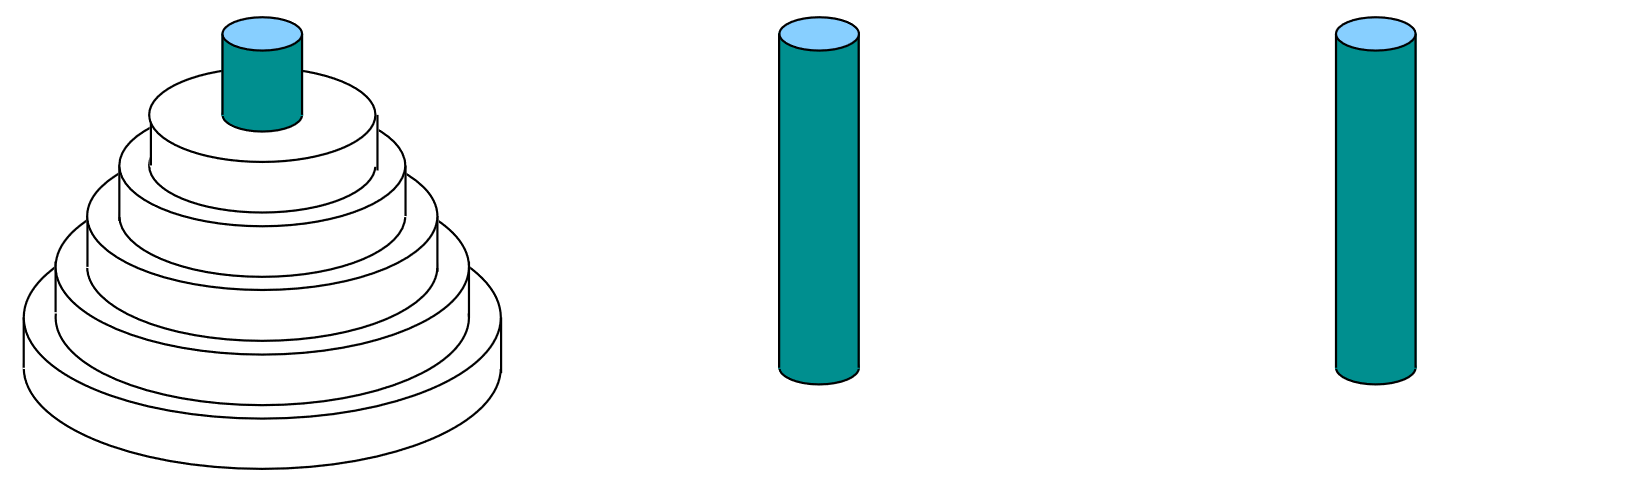
\includegraphics[width=\textwidth]{torensVanHanoi}
		\caption{De torens van Hanoi.}
		\label{fig:torensVanHanoi}
	\end{figure}
	\begin{itemize}
		\item Twee niveaus van positieve uitspraken:
		\begin{enumerate}
			\item Nuldeordepredicaten: Dit zijn strings, zoals \textit{DeLuchtIsBlauw} of \textit{Veilig}.
			\item Eersteordepredicaten: Deze zijn functies met een aantal parameters, die objecten aanduiden.
		\end{enumerate}
		\item Elke schijf hangt aan een bepaalde pin, er kan dus een predicaat van de eerste orde ingevoerd worden zoals bijvoorbeeld:
		$$\texttt{HangtAan(schijf1, pin1)}$$
		\item Ook moet duidelijk gemaakt worden dat twee verschillende pinnen effectief verschillend zijn:
		$$\texttt{IsNiet(pin1, pin2)}$$
		\item De begintoestand van de torens van Hanoi kan nu beschreven worden als volgt:
		\begin{equation*}
			\begin{split}
				\texttt{HangtAan(schijf1, pin1)}& \;\wedge \\
				\texttt{HangtAan(schijf2, pin1)}& \;\wedge \\
				\texttt{HangtAan(schijf3, pin1)}& \;\wedge \\
				\texttt{HangtAan(schijf4, pin1)}& \;\wedge \\
				\texttt{HangtAan(schijf5, pin1)}& \;\wedge \\
				\texttt{IsNiet(pin1, pin2)}& \;\wedge \\
				\texttt{IsNiet(pin1, pin3)}& \;\wedge \\
				\texttt{IsNiet(pin2, pin1)}& \;\wedge \\
				\texttt{IsNiet(pin2, pin3)}& \;\wedge \\
				\texttt{IsNiet(pin3, pin1)}& \;\wedge \\
				\texttt{IsNiet(pin3, pin2)}&  \\
			\end{split}
		\end{equation*}
		De predicaten worden gebonden met een logische EN. Ook is het nodig om de symmetrie te definiëren, aangezien STRIPS hier niets van af weet.
		\item Nu kan een actie gedefinieerd worden om een schijf te bewegen. Voor elke schijf moet dit apart gedaan worden. Hier wordt het uitgewerkt voor schijf 2:
		\begin{equation*}
			\begin{split}
				\texttt{Beweeg}&\texttt{Schijf2(van, naar, tussen)}: \\ 
				P : &\quad\texttt{IsNiet(van, naar)} \wedge \texttt{IsNiet(van, tussen)} \wedge \texttt{IsNiet(naar, tussen)}  \\
				    &\quad \texttt{HangtAan(schijf1, tussen)} \wedge \texttt{HangtAan(schijf2, van)} \\
				+ : &\quad \texttt{HangtAan(schijf2, naar)}\\
				- : &\quad \texttt{HangtAan(schijf2, van)}
			\end{split}
		\end{equation*}
		Elke actie bestaat uit een premisse $P$ die voldaan moet zijn vooraleer de actie kan uitgevoerd worden. De lijst van de toe te voegen uitspraken wordt aangeduid met het $+$ symbool en de lijst met de te verwijderen uitspraken worden aangeduid met het $-$ symbool.
		\item Om de symmetrie van de begintoestand op te lossen zou een actie \texttt{IsSymmetrie(A, B)} aangemaakt kunnen worden als volgt:
		\begin{equation*}
			\begin{split}
				\texttt{IsSym}&\texttt{metrie(A, B)}: \\ 
				P : &\quad \texttt{IsNiet(A, B)}\\
				+ : &\quad \texttt{IsNiet(B, A)}\\
				- : &\quad /
			\end{split}
		\end{equation*}
	\end{itemize}
\end{itemize}
\section{Efficiënt zoeken in zoekruimten}
\subsection{Breedte-eerst zoeken}
\begin{itemize}
	\item De \textbf{vertakkingsfactor} is het gemiddeld aantal nieuwe, nog niet bekeken buren van een onderzochte knoop en wordt voorgesteld door $b$ (branching factor).
	\item Bij de torens van Hanoi is $b \approx 1,5$.
	\item Voor een diepte $d$ worden ongeveer 
	$$1 + b + b^2 + ... + b^d = \frac{b^{d + 1} - 1}{b - 1}$$
	knopen bezocht. Voor $b$ voldoende groter dan $1$ is dit ongeveer $b^d$.
	\item Als we tien zetten voor elke speler willen vooruitkijken bij schaken, moeten er $6^{20} \approx 3.6\cdot10^{15} = 3,6$ biljard knopen ontwikkeld worden.
	\item Indien zowel start- als eindtoestand bekend zijn, kan \textbf{bidirectioneel zoeken} toegepast worden. Er wordt vooruit gezocht vanuit het startpunt, en achteruit vanuit het doel, beide met breedte-eerst zoeken. Er moet dan in plaats van $b^d$ knopen slechts $2b^{d/2}$ knopen ontwikkeld worden. Voor $b = 2$ en $d = 20$ krijgen we met breedte-eerst zoeken $10^6$ knopen en met bidirectioneel zoeken ongeveer 2000.
\end{itemize}
\subsection{Heuristieken}
In plaats van breedte-eerst zoeken te gebruiken zou ook een manier kunnen gebruikt worden die de meest interessante knoop volgt, in plaats van ze blindelings af te lopen.
\begin{itemize}
	\item Bij het zoeken in een graaf worden er aan elke knoop $k$ twee waarden toegekend:
	\begin{enumerate}
		\item De gekende kost $g(k)$ van de knoop: 
		\begin{itemize}
			\item Deze functie is een schatting van de werkelijke kost $g^*(k)$ van het kortste  pad van de startknoop naar $k$.
			\item Het wordt berekend door bij de kost van zijn voorganger $v$ de kost $c(v \rightarrow k)$ op te tellen; de kost van de actie die $v$ omzet in $k$.

			\item Er geldt steeds $g(k) \geq g^*(k)$.
		\end{itemize} 
		\item De heuristische kost $h(k)$ van de knoop:
		\begin{itemize}
			\item Deze functie is een schatting van $h^*(k)$, de kost om vanuit de knoop het doel te bereiken via het kortste pad.
		\end{itemize}
	\end{enumerate}
	\item De som van deze twee waarden geven de geschatte kost, verpakt door de evaluatiefunctie $f$:
	$$f(k) = g(k) + h(k)$$
	\alert Interessante knopen heben een lage $f$ waarde. 
	\item \textbf{Beste-eerst zoeken}:
	\begin{enumerate}
		\item[(1)] Steek de startknoop $s$ in de verzameling niet-ontwikkelde knopen NOK met $g(s) = 0$. Geef alle andere knopen een voorlopige schatting $g(k) = \infty$.
		\item[(2)] Als NOK leeg is stop dan zonder oplossing, ga anders naar (3).
		\item[(3)] Zoek de knoop $k$ uit NOK met de laagste evaluatiewaarde en verwijder hem uit NOK.
		\item[(4)] Als $k$ in het doel zit, geef het pad naar $k$ terug en stop; ga anders naar (5).
		\item[(5)] Voor elke buur $b$ van $k$: bereken $g_k(b) = g(k) + c(k \rightarrow b)$ en vergelijk $g_k(b)$ met de voorlopige waarde die $g(b)$ al gekregen had. Als $g_k(b) < g(b)$, vervang dan $g(b)$ door $g_k(b)$ en steek $b$ in NOK als $b$ daar niet in zit.
		\item[(6)] Ga terug naar (2).
	\end{enumerate}
	\item De functie $g$ is afhankelijk van het probleem, maar $h$ hoeft dit niet te zijn. Er zijn verschillende mogelijkheden voor $h$. Er is wel de voorwaarde dat ze \textbf{toelaatbaar} moeten zijn. Dit wil zeggen dat het een pad vindt en dat dit pad optimaal is.
\end{itemize}
\subsubsection{A* heuristieken}
\begin{itemize}
	\item Een heuristiek is $A*$ als $h(k) \leq h^*(k)$.
	\item \underline{Bewijs:} indien er slechts een eindig aantal knopen $k_i$, met $g^*(k_i) \leq g^*(D)$ zijn, is een $A*$-heuristiek toelaatbaar.
	\begin{itemize}
		\item Neem een $A*$ heuristiek $h$ en bewijs dat er steeds een knoop $k'$ is die voldoet aan de volgende voorwaarden:
		\begin{enumerate}
			\item[(1)] $k'$ zit in NOK.
			\item[(2)] $k'$ ligt op een optimaal pad van $s$ naar $D$.
			\item[(3)] De schatting $g(k')$ is correct: $g(k') = g^*(k')$.
		\end{enumerate}
	\item Dit is geldig indien $k'$ de startknoop is. Er is minstens één buur $k''$ die ook op het optimale pad ligt. Door $k'$ te ontwikkelen wordt zijn plaats ingenomen door zijn opvolger $k''$ op het optimale pad.  $k''$ voldoet aan (3), want
	$$g^*(k'') = g(k') + c(k' \rightarrow k'') = g_{k'}(k'')$$
	\item Als $k'$ de laatste knoop op het pad is die aan de voorwaarden voldoet dan is de nieuwe $g(k'')$-waarde kleiner dan de vorige en komt $k''$ zeker in NOK. Bovendien geldt
	
	$$f(k') = g(k') + h(k') \leq g^*(k') + h^*(k') = g^*(D)$$
	
	\item Er kan geen enkele $k$ ontwikkeld worden met $g(k) > g^*(D)$, want dan zou $f(k) > f(k')$ zijn.
	\item Iedere keer als een knoop $k$ ontwikkeld wordt, is er een kleinere waarde voor $g(k)$ die overeenkomt met de kost van een pad $s$ naar $k$.
	\item Ooit zal een doelknoop $d$ gekozen worden voor ontwikkeling en die heeft $g(d) = f(d) \leq g^*(D)$, en is bijgevolg optimaal.
	\end{itemize}
\end{itemize}

\subsubsection{Monotone heuristieken}
\begin{itemize}
	\item Een heuristiek is monotoon als 
	\begin{enumerate}
		\item voor elk paar knopen geldt dat $h(v) - h(k) \leq c(v \rightarrow k)$.
		\item $h(d) = 0$ voor alle $d$ in de doelverzameling $D$.
	\end{enumerate}
	\item \underline{Bewijs:} Neem een willekeurig pad $k_0k_1, ...,k_n$ tussen twee knopen $k_0$ en $k_n$. Dan is de functie $g(k_i) + h(k_i)$ monotoon stijgend als functie van $i$. Hierin wordt $g(k_i)$ gerekend langs het pad vanaf het startpunt $k_0$.
	\begin{itemize}
		\item Voor $i < n$ geldt dat $g(k_i) + c(k_i \rightarrow k_{i + 1}) = g(k_{i + 1})$
		\item Ook geldt er dat $h(k_i) \leq h(k_{i + 1}) + c(k_i \rightarrow k_{i + 1})$.
		\item Deze twee termen optellen en de term $c(k_i \rightarrow k_{i + 1})$ schrappen levert 
		$$g(k_i) + h(k_i) \leq g(k_{i + 1}) + h(k_{i + 1})$$
	\end{itemize}
	\item \underline{Twee gevolgen:}
	\begin{enumerate}
		\item Een monotone heuristiek is $A*$.
		\item Een knoop $k$ wordt nooit ontwikkeld voor $g^*(k)$ gekend is.
	\end{enumerate}
	\item Efficiëntie
	\begin{itemize}
		\item Voor $h = 0$ krijgen we breedte-eerst zoeken.
		\item Voor $h = h*$ krijgen we de optimale heuristiek, die rechtstreeks naar het doel leidt, en die ook monotoon is.
		\item Hoe bepalen of een willekeurige monotone heuristiek beter is dan een andere?
		\begin{itemize}
			\item Laatste ontwikkelde knoop is altijd $d$ met $g^*(d) = g^*(D)$ en $h(d) = 0$.
			\item Voor een monotone heuristiek moeten alle knopen ontwikkeld worden waarvoor $g^*(k) + h(k) < g^*(D)$, en geen enkele waarvoor $g^*(k) + h(k) > g^*(D)$.
			\item Een monotone heuristiek $h_1$ ontwikkelt minder knopen dan een monotone heuristiek $h_2$ als $h_1(k) > h_2(k)$. 
			\item Als voor sommige $k$ geldt dat $h_1(k) < h_2(k)$ en voor andere $k$ $h_1(k) > h_2(k)$, kan een betere heuristiek opgebouwd worden:
			
			$$h_3 = \max\{h_1(k), h_2(k)\}$$
		\end{itemize}
		
	\end{itemize}
\end{itemize}

\subsubsection{Relaxatieheuristieken}
\begin{itemize}
	\item Worden bekomen door het originele probleem sterk te vereenvoudigen.
	\item Er worden verbindingen toegevoegd in de graaf, wat overeenkomt met het schrappen van acties in de premisse.
	\item Het kortste pad in nieuwe graaf is zeker niet langer dan het kortste pad in de originele graaf. Deze heuristiek is dan ook $A^*$.
\end{itemize}

\section{Spelbomen}
\begin{itemize}
	\item Wat doen indien er geen volledige kennis is over het resultaat van acties?
	\item Een \textbf{nulsomspel} (Engels: two player zero sum game)
	\begin{itemize}
		\item Twee spelers.
		\item Enkel winst mogelijk ten koste van de andere speler.
		\item De winst van de ene speler is gelijk aan het verlies van de andere speler.
		\item Elke speler probeert zijn winst te maximaliseren.
	\end{itemize}
	\item \underline{Voorbeeld van een nulsomspel:}
	\begin{itemize}
		\item Op een tafel tussen twee spelers liggen een aantal stapels jetons.
		\item De speler die aan de zet is moet een stapel nemen, en deze verdelen in twee ongelijke stapels.
		\item De speler die niet meer kan zetten verliest.
		\item De winnaar krijgt als winst het aantal punten gelijk aan het aantal overblijvende stapels, en de verliezer verliest dan ditzelfde aantal punten.
		\item Er kan een bijhorende boom (figuur \ref{fig:spelboom}) opgesteld worden die alle mogelijke zetten beschrijft.
		\begin{figure}
			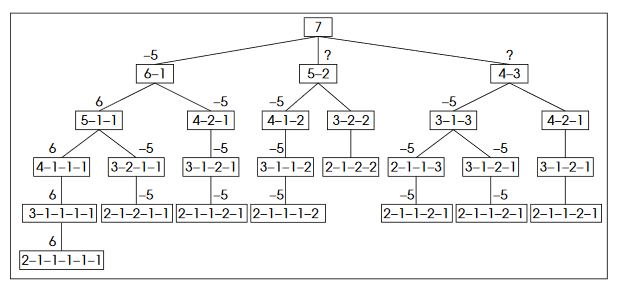
\includegraphics[width=\textwidth]{spelboom}
			\caption{Een spelboom waarbij de startsituatie een stapel van 7 jetons is.}
			\label{fig:spelboom}
		\end{figure}
		\item Noem de speler die begint \textit{Max}, en de andere speler \textit{Min}.
		\item Bij elke eindpositie is de winst of verlies van Max berekent.
		\item De overige posities kunnen van onder naar boven opgesteld worden:
		\begin{enumerate}
			\item Als Max aan zet is dan nemen we de grootste score.
			\item Als Min aan zet is nemen we de kleinste score.
		\end{enumerate} 
		\item Dit heet \textbf{minimax}. 
		\item Er wordt gebruik gemaakt van \textbf{$\alpha-\beta$ snoeien} om oninteressante zetten (deelbomen) zeker niet te evalueren in de spelboom. Op die manier is er minder geheugen nodig.
		\begin{itemize}
			\item De zet $7\rightarrow6-1$ levert een score van $-5$ op.
			\item Van de zet $7\rightarrow5-2$ weten we niet wat de score is.
			\begin{itemize}
				\item We weten wel dat Min erop kan reageren met een zet die een score van $-5$ geeft.
				\item Het kan zijn dat de andere deelboom een betere score oplevert voor Min, maar het zal zeker geen lagere zijn (want die zet zou hij niet nemen).
				\item Deze zet is niet beter dan $7\rightarrow 6 - 1$	
		\end{itemize}
			\item Algemeen wordt er gezocht naar een pad naar een blad waarbij zowel Max als Min steeds de beste zet kiezen.
			\begin{itemize}
				\item Op dit pad is de kost van alle knopen gelijk.
				\item De kost is $s_{opt}$, de optimale score.
			\end{itemize}
		\end{itemize}
		\item Moeten alle knopen ge-evalueerd worden om de optimale score te vinden?
		\begin{itemize}
			\item Een \textbf{voorbroer} $b$ van een knoop $k$ is een broer van $k$, of een broer van één van de voorouders van $k$ (Figuur \ref{fig:voorbroers}).
			\begin{figure}
				\centering
				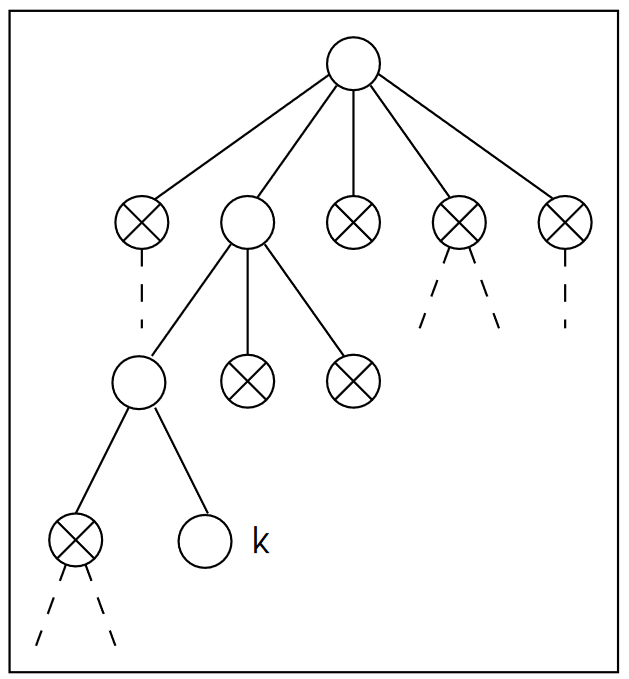
\includegraphics[width=0.5\textwidth]{voorbroers}
				\caption{De voorbroers van een knoop $k$ worden gemarkeerd met een kruis.}
				\label{fig:voorbroers}
			\end{figure}
			\item Neem een knoop $k$ en veronderstel dat $s(k)$ kan vervangen worden door een schatting $f$.
			\item De waarden van de voorouders van $k$ kunnen ook nu veranderd worden. Stel $f > s(k)$:
			\begin{enumerate}
				\item $k$ is een minknoop. Als $f >  s(b)\;\forall\;b \hbox{ broer van } k$, dan wordt de $s$-waarde van de ouderknoop vervangen door $f$. Nu wordt naar geval 2 gegaan.
				\item $k$ is een maxknoop en geen wortel. De nieuwe $s-$waarde van de ouder is hoogstens $f$. Nu wordt naar geval 1 gegaan.
			\end{enumerate}
		\end{itemize}
	\end{itemize}
\end{itemize}
\chapter{Expertsystemen}
\begin{itemize}
	\item Kennis van een \textbf{echte expert} overnemen in een programma.
	\item De \textbf{gebruiker} moet ook enigszins kennis hebben. Hij moet de conclusies begrijpen en toepassen.
	\item \textbf{MYCIN}: een expertsysteem om te helpen bij de diagnose van bepaalde besmettelijke bloedziekten.
	\begin{itemize}
		\item Is in staat om een betere diagnose te stellen dan een arts die geen expert is in het gebied.
		\item De gebruiker moet wel een arts zijn die de diagnose begrijpt.
	\end{itemize}
	\item Een expertsysteem maakt gebruik van \textbf{vuistregels}, waarop later nog \textbf{verfijningen} ingevoerd worden:
	\begin{enumerate}
		\item werken met \textbf{onzekere conclusies}. Dit wordt ingevoerd om contradicties te behandelen indien deze voorkomen.
		\item De invoering van \textbf{frames}. Zorgt voor een betere orderning voor grote hoeveelheden kennis.
	\end{enumerate}
\end{itemize}
\section{Eenvoudige systemen}
\begin{itemize}
	\item Een expertsysteem bestaat uit \underline{twee hoofdcomponenten}
	\begin{enumerate}
		\item Een \textbf{kennisbank}:
		\begin{itemize}
			\item bevat \textbf{feiten}: dit zijn uitspraken die waar zijn.
			\item bevat \textbf{regels}: dit heeft de vorm \textbf{als$<$premisse$>$dan$<$conclusie$>$}
			\regel{AS=rond \textbf{en} MATERIAAL=staal}{SMERING=olie}
		\end{itemize}
		\item Een \textbf{afleidingssysteem}:
		\begin{itemize}
			\item Elk probleem bestaat uit begingegevens en een doel.
			\item Deze gegevens vormen een lijst van feiten die gekend zijn.
			\item Het doel is ook een lijst van uitspraken.
			\item Het doel is bereikt als één uitspraak uit de lijst is afgeleid uit de gegevens.
		\end{itemize}
	\end{enumerate}
	\item Het afleidingssysteem kan op \underline{twee manieren} werken.
	\begin{itemize}
		\item \textbf{Forward chaining:}
		\begin{itemize}
			\item Kan in $O(g)$, met $g$ de grootte van de regelbank.
			\item Twee gegevensstructuren:
			\begin{itemize}
				\item \textbf{LijstMetRegels($u$)} die voor elke uitspraak $u$ bijhoudt in welke regels ze in de premisse voorkomt.
				\item \textbf{Premisseteller($r$)} die voor elke regel $r$ bijhoudt hoeveel uitspraken in de premisse nog niet gevalideerd zijn.
			\end{itemize}
			\item Werking:
			\begin{enumerate}
				\item Initialiseer de gegevensverzameling en de doelverzameling.
				\item Voor elke regel $r$, initialiseer \textit{Premisseteller($r$)}
				 op het aantal uitspraken in de premisse.
				\item Zolang de gegevensverzameling en het doel geen gemeenschappelijk element bevatten, en de gegevensverzameling niet leeg is:
				\begin{enumerate}
					\item Neem een uitspraak $u$ uit de gegevensverzameling.
					\item Voor elke regel $r$ in \textit{LijstMetRegels($r$)}, verminder \textit{Premisseteller($r$)}. Als deze daardoor nul wordt, zet elke uitspraak uit de conclusie die nog niet behandeld is in de gegevensverzameling.
				\end{enumerate}
				\item Deel het resultaat mee aan de gebruiker.
			\end{enumerate}
			\item \underline{Voorbeeld:}
			\begin{itemize}
				\item Stel volgende regelbank:
				
				\noindent\fbox{%
					\parbox{\linewidth}{%
						\regel{$X$ kwettert en $X$ zingt}{$X$ is een kanarie}
						\regel{$X$ kwaakt en $X$ eet vliegen}{Dan $X$ is een kikker}
						\regel{$X$ is een kikker}{$X$ is groen}
						\regel{$X$ is een kanarie}{$X$ is geel}
					}%
				}


				\item Stel nu dat we een huisdier hebben, Fritz,  en er zijn twee dingen bekend over hem: hij kwaakt en eet vliegen. We willen nu de kleur weten.
				\item Fritz wordt gesubstitueerd voor $X$ in regel 1, maar hij voldoet niet aan de premisse. Hij wordt nu gesubstitueerd voor $X$ in regel 2, zodat er besloten wordt dat hij een kikker is. Dit wordt dan toegevoegd aan de gegevens. We weten nu dat Fritz kwaakt, dat hij vliegen eet en dat hij een kikker is.
				\item Fritz kan nu gesubstitueerd worden in regel 3, zodat er besloten wordt dat hij groen is.
			\end{itemize}
			\item Forward Chaining werkt van links naar rechts, startend vanaf de gekende feiten om tot een conclusie te komen.
			\alert In het algoritme kunnen regels toegepast worden die uiteindelijk niet bijdragen tot de oplossing. Men probeert dit efficiënter op te lossen met backwards chaining.
		\end{itemize}
		\item \textbf{Backward chaining:}
		\begin{itemize}
			\item Kan in $O(g)$, met $g$ de grootte van de regelbank.
			\item Werking:
			\begin{enumerate}
				\item[$A.$] Behandeling voor een regel waarbij alle uitspraken uit de premisse gegevens zijn:
				\begin{enumerate}
					\item[$A1.$] Voeg alle uitspraken uit de conclusie toe aan de gegevens.
					\item[$A2$] Voor alle tussenregels voor wie, op deze manier, alle uitspraken uit de premisse gegevens zijn geworden, behandel ze volgens $A$.
					\item[$A3.$] Verwijder de regel uit de regelbank of uit de verzameling tussenregels.
				\end{enumerate}
				\item[$B.$] Behandeling voor een regel waarbij niet alle uitspraken uit de premisse gegevens zijn:
				\begin{enumerate}
					\item[$B1.$] Voeg alle uitspraken uit de premisse die geen gegevens zijn toe aan de tussendoelverzameling.
					\item[$B2.$] Verwijder de regel uit de regelbank en voeg hem toe aan de tussenregels.
				\end{enumerate}
				\item[$C.$] Oplossingsalgoritme:
				\begin{enumerate}
					\item Initialiseer de gegevensverzameling en doelverzameling. Initialiseer ook de verzamelingen van tussendoelen en tussenregels: deze zijn leeg.
					\item Zolang er geen resultaat is gevonden, en er een regel is uit de regelbank wiens conclusie een doel of een tussendoel bevat, doe het volgende:
					\begin{enumerate}
						\item Neem zo een regel.
						\item Als alle uitspraken uit de premisse gegevens zijn, behandel volgens $A$, anders volgende $B$.
					\end{enumerate}
				\end{enumerate}
			\end{enumerate}
			\item \underline{Voorbeeld:}
			\begin{itemize}
				\item Veronderstel dezelfde regelbank als bij forward chaining.
				\item Stel nu dat we een huisdier hebben, Fritz,  en er zijn twee dingen bekend over hem: hij kwaakt en eet vliegen. We willen nu de kleur weten.
				\item Fritz wordt gesubstitueerd voor $X$ in regel 3. Men moet dan bewijzen dat Frits een kikker is.
			\end{itemize}
		\end{itemize}
	\end{itemize}
\end{itemize}
\section{De constructie van een expertsysteem}
\begin{itemize}
	\item \underline{Twee soorten kennis nodig:}
	\begin{itemize}
		\item Kennis over het probleemgebied. Experten in het toepassingsgebied weten hoe ze problemen moeten oplossen, maar kunnen deze kennis niet vertalen in de vorm die een expertsysteem nodig heeft.
		\item Kennis over expertsystemen. Een team die de kennis van de experten kan filteren en omvormen naar de juiste vorm. 
	\end{itemize}
\end{itemize}
\section{Onzekerheid}
\begin{itemize}
	\item De relatie tussen premisse en conclusie van een regel is niet altijd zeker.
	\item \underline{Voorbeeld:}
	\begin{itemize}
		\item Een expertsysteem dat de oorzaak zoekt van problemen in een computer. Dit systeem kan een reparateur begeleiden die een defecte computer moet repareren.
		\item De reparateur moet melden wat de symptomen zijn. Het systeem moet de actie bepalen die moet ondernomen worden om het probleem op te lossen. Mogelijke regels zijn bijvoorbeeld:
		\regel{SYMPTOOM=computer doet niets bij opstarten}{PROBLEEM=voeding defect}
		\regel{SYMPTOOM=voeding defect}{PROBLEEM=vervang voeding}

		
		\item Maar soms kan een probleem meerdere oorzaken hebben, waarbij sommige meer waarschijnlijkheid hebben dan anderen:
		\regel{PROBLEEM=bootloader hangt}{OORZAAK=schijf defect \textbf{of} OORZAAK=bootloaderinstallatie \textbf{of} ...}

		
		\item Er wordt dan een numerieke factor toegekend, die de waarschijnlijkheid aanduidt. 
		
		\item \textbf{Hoe wordt de numerieke waarde bepaalt?}
		\begin{enumerate}
			\item Vage verzamelingen: \textbf{Niet te kennen}.
			\item Bayesiaans redeneren: 
			\begin{itemize}
				\item Stel volgende regels:
				\regel{het regent op dag x}{is de kans dat het op dag x + 1 regent 0,8}
				\regel{het niet regent op dag x}{is de kans dat het op dag x + 1 regent 0,3}

				\item Statistisch redeneren kan toegepast worden in expertsystemen als er voldoende statistische informatie is:
				\begin{itemize}
					\item De kans dat het morgen en overmorgen regent: $0,8 \times 0,8 = 0,64$.
					\item Da kans dat het morgen niet regent, maar overmorgen wel: $0,2 \times 0,3 = 0,06$.
				\end{itemize}
				\item Stel dat we nu twee uitspraken $a$ en $b$ hebben met $p(a) = 0,8$ en $p(b) = 0,2$.
				\item Wat is de kans op $p(a\; \hbox{\textbf{en}}\;b)$? Deze waarde kan tussen 0 en 0,2 liggen. 
				
				Als $a = $ het regent morgen en $b = $ het regent niet morgen, dan is $p(a\; \hbox{\textbf{en}}\;b) = 0$. 
				
				Als $a = $ het regent morgen en $b = $ het regent morgenochtend, dan is $p(a\; \hbox{\textbf{en}}\;b) = 0,2$
				
				\alert Bayesiaans redeneren is geen aangewezen methode.
			\end{itemize}
			\item Theorie van zekerheidsfactoren:
			\begin{itemize}
				\item Er wordt een zekerheidsfactor berekent op basis van woorden die een expert uitdrukt:
				\begin{table}[h]
					\centering
					\begin{tabular}{| l | c |}
						\hline 
						Term & zekerheidsfactor \\
						\hline 
						zeker niet & -1,0 \\
						bijna zeker niet & -0,8 \\
						waarschijnlijk niet & -0,6 \\
						misschien niet & -0,2 tot +0,2 \\
						misschien & +0,4 \\
						waarschijnlijk & +0,6 \\
						bijna zeker & +0,8 \\
						zeker & +1,0 \\
						\hline
					\end{tabular}
				\end{table}
			
				\item Voor een uitspraak $a$ wordt de zekerheidsfactor van die uitspraak $z(a)$. Hierbij geldt $z(a) = -z(\neg a)$.
				
				\item Hoe berekenen van de zekerheid van een conclusie als de premisse van een regel zelf onzeker is?
				
				\begin{itemize}
					
					\item[] \noindent\fbox{%
						\parbox{\linewidth}{%
							\begin{equation*}
							\begin{split}
							& \hbox{\textbf{als} b} \\
							& \hbox{\textbf{dan} a \qquad (x)}  
							\end{split}
							\end{equation*}
								$$z(a) = z(b) \times x$$
						}%
					}
		
					\item[]
					\noindent\fbox{%
						\parbox{\linewidth}{%
						\begin{equation*}
						\begin{split}
						& \hbox{\textbf{als} b \textbf{en} c \textbf{en} d} \\
						& \hbox{\textbf{dan} a \qquad (x)}  
						\end{split}
						\end{equation*}
					$$z(b\;\hbox{\textbf{en}}\;c\; \hbox{\textbf{en}}\;d) = \min(z(b), z(c), z(d)) \times x$$
						}%
					}
					
					
				
					\item[] \noindent\fbox{%
						\parbox{\linewidth}{%
						\begin{equation*}
						\begin{split}
						& \hbox{\textbf{als} e} \\
						& \hbox{\textbf{dan} a \qquad (x)}  
						\\[3ex]
						& \hbox{\textbf{als} f} \\
						& \hbox{\textbf{dan} a \qquad (y)}  
						\end{split}
						\end{equation*}
						$$z_1 = z(e) \times x,\qquad z_2 = z(f) \times y$$
						$$z(a) = \frac{z_1 + z_2}{1 - \min(|z_1|, |z_2|)}$$
						
							
						}%
					} 
		
				\end{itemize}
			\end{itemize}
		\end{enumerate}	
	\end{itemize}
\end{itemize}

\section{Frames en regelschema's}
\begin{itemize}
	\item Noodzaak om kennis in te delen.
	\item Een \textbf{frame} kan vergeleken worden met een klasse uit object georiënteerde programeertalen.
	\item Komt uit de theorie van \textbf{semantische netten}.
	\begin{figure}[ht]
		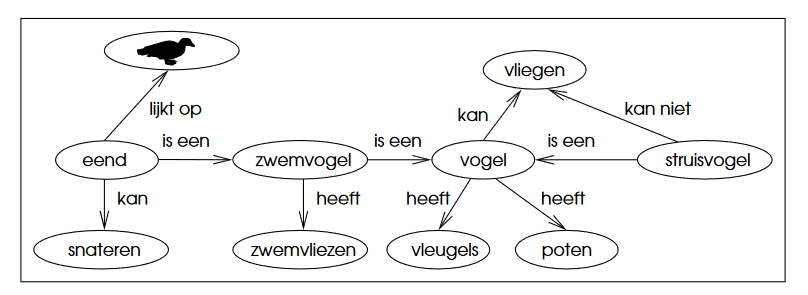
\includegraphics[width=\textwidth]{semantisch_net}
		\caption{Een semantisch net.}
	\end{figure}
	\begin{itemize}
		\item Een semantisch netwerk bestaat uit een gelabelde gerichte multigraaf.
		\item Elke knoop is een begrip, en elk begrip is verbonden met andere begrippen.
	\end{itemize}
	\item Opzoeken van informatie:
	\begin{itemize}
		\item \textit{Kan een eend snateren?} Vanuit 'eend' wordt de 'kan'-relatie naar 'snateren' genomen. Het antwoord is 'ja'.
		\item \textit{Heeft een eend zwemvliezen?} Via de 'is een'-relatie weet men dat een eend een zwemvogel is. De zwemvogel bevat een 'heeft'-relatie naar 'zwemvliezen'. Het antwoord is 'ja'.
		\item \textit{Heeft een eend vleugels?} Via de twee 'is een'-relaties weet men dat een eend een vogel is. Een vogel bevat een 'heeft'-relatie naar 'vleugels'. Het antwoord is 'ja'.
		\item \textit{Eet een eend sla?} Na het netwerk te hebben afgezocht is er geen verband tussen sla en eenden gevonden.
		
	\end{itemize}
	\item Twee regels om informatie op te zoeken:
	\begin{enumerate}
		\item Volg de takken waarvan de naam in de vraag staat.
		\item Volg de takken met 'is een' als naam. Deze zorgt ervoor dat het probleem veralgemeend wordt (eend wordt zwemvogel en dan vogel), maar het wordt enkel gebruikt als er geen andere informatie meer beschikbaar is via andere relaties.
	\end{enumerate}
	\item \textit{Kan een struisvogel vliegen?}  We vinden informatie met de 'kan niet'-relatie zodat het antwoord 'nee' is. 
	\alert Het net bevat enkel informatie en geen regels voor de verwerking ervan.
	\item Frames versus objectgeoriënteerd programmeren:
	\begin{enumerate}
		\item Ze hebben beiden een hiërarchisch systeem dat gebruik maakt van (geen meervoudige) overerving.
		\item In een semantisch net wordt er geen onderscheid gemaakt tussen klassen en objecten.
	\end{enumerate}
	
\end{itemize}
\chapter{De regel van Bayes en Markovketens}


\section{Probabiliteit}
\begin{itemize}
	\item Een universum $U$ met een eindig aantal toestanden.
	\item De kans op een uitspraak $a$ wordt genoteerd als $p(a)$ en is gelijk aan:
	
	$$p(a) = \frac{\#(a)}{\#U} $$
	met $\#U$ het aantal toestanden in het universum en $\#(a)$ het aantal toestanden waarin $a$ waar is binnen dit universum.
	\begin{itemize}
		\alert Niet bruikbaar: het systeem kan enkel de kans bepalen van reeds bestaande gevallen. 
		\begin{enumerate}
			\item \begin{itemize}
				\item Stel $83$-jarige patiënt met hoofdpijn.
				\item In het universum zit er een $83$-jarige patiënt met hoofdpijn.
				\item De patiënt kan dus niet bestaan.
			\end{itemize}
			\item \begin{itemize}
				\item Stel $43$-jarige patiënt die niet rookt en metselaar is.
				\item In het universum zit één metselaar die $43$ jaar is, niet rookte en psoriasis heeft. 
				\item De patiënt heeft dus psoriasis.
			\end{itemize}
		\end{enumerate}
		
	\end{itemize}
	\item Er is een \textbf{zinvolle veralgemening} nodig.
	\item Het lerend programma moet een \textbf{model} gebruiken waarbij een aantal parameters moet worden ingevuld. 
	\item De waarden van de parameters van dit model kan een zinnige veralgemening geven van probailiteit, via \textbf{de regel van Bayes}.
		
\end{itemize}


\section{De regel van Bayes}
\begin{figure}[t]
	\centering
	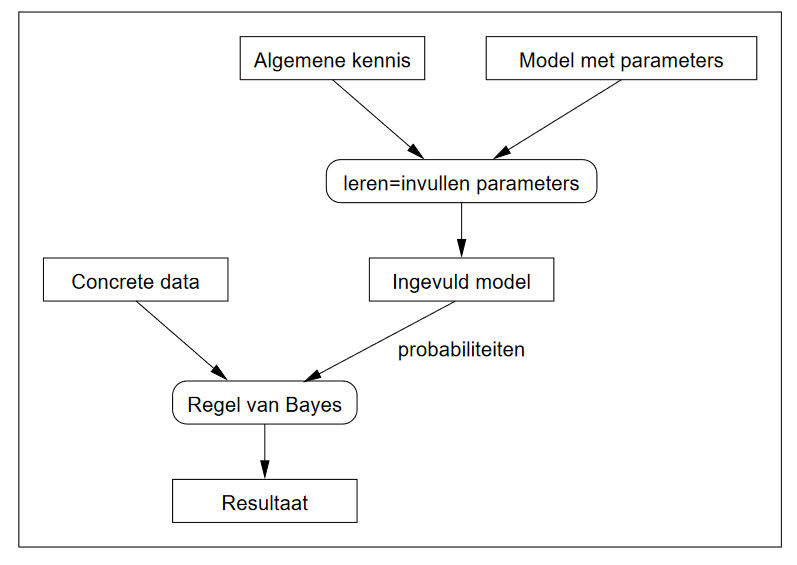
\includegraphics[width=\textwidth]{de_regel_van_bayes}
	\caption{De regel van Bayes bij artificiële intelligentie.}
\end{figure}
\begin{itemize}
	\item De voorwaardelijke kans $p(a|b)$ is de kans dat $a$ waar is gegeven dat $b$ waar is.
	\item Stel $\#U$ het aantal toestanden in het universum en $\#(a)$ het aantal toestanden waarin $a$ waar is:
	
	$$p(a) = \frac{\#(a)}{\#U}, \qquad p(a|b) = \frac{p(a\& b)}{p(b)} = \frac{\#(a\& b)}{\#(b)}$$
	
	\item Dit kan herschreven worden:
	$$p(b)p(a|b) = p(a\& b)$$
	
	zodat 
	$$p(a\& b) = p(b \& a)$$
	
	of 
	
	$$p(b)p(a|b) = p(a)p(b|a)$$
	
	\item \underline{Voorbeeld:} 
	\begin{itemize}
		\item Universum = 10.000 vogels
		\item 1.000 van deze vogels zijn raven: $p(raaf) = 0,1$
		\item 2 van deze vogels zijn wit: $p(wit) = 0,0002$
		\item Er is slechts 1 witte raaf: $p(raaf|wit) = 0,5$ en $p(wit|raaf) = 0,001$ 
		
		\item \textbf{Dus:} $p(wit)p(raaf|wit) = p(raaf)p(wit|raaf) = 0,0001$
	\end{itemize}
	\item Dit kan veralgemeend worden met \textbf{de regel van Bayes}:
	
	$$p(a|b) = \frac{p(a)p(b|a)}{p(b)}$$
	
	\item Veronderstel hypothetische uitspraken $h_i, i = 1, 2, ...$.
	\begin{itemize}
		\item Voor een willekeurig item is exact één hypothetische uitspraak waar.
		\item Het resultaat van een aantal metingen op dat item resulteren in een uitspraak $d$.
		\item Wat is de kans dat een hypothese $h_i$ waar is gegeven de data $d$?
		
		$$p(h_i|d) = \frac{p(h_i)p(d|h_i)}{p(d)}$$
	\end{itemize}
	\item \underline{Voorbeeld:}
	\begin{itemize}
		\item Er is een groot aantal ziektes.
		\item Deze leiden tot de lijst van hypothesen, waarbij $h_i$ staat voor de uitspraak "De patiënt heeft de $i-$de ziektepatroon".
		\item Is er een groot aantal mogelijke symptomen.
		\item Bij een patiënt kunnen de symptomen vastgesteld worden, die resulteren in een uitspraak $d$.
		\item Hoe bepalen welk ziektepatroon het meest waarschijnlijk is?
		\begin{itemize}
			\item $p(h_i)$ is de kans dat ziektepatroon $i$ voorkomt in het universum. Dit is verondersteld gekend te zijn.
			\item $p(d|h_i)$ is de kans dat ziektepatroon $i$ de opgegeven symptomen veroorzaakt. Dit is verondersteld gekend te zijn.
			\item $p(d)$ kan berekend worden uit de vorige gegevens, als er verondersteld wordt dat er bij elke patiënt juist één $i$ is waarvoor $h_i$ waar is:
			
			$$p(d) = \sum_i p(h_i\&d) = \sum_i p(h_i)p(d|h_i)$$
			
			\item De expliciete waarde van $p(d)$ is eigenlijk niet nodig. 
		\end{itemize}
	\end{itemize}
	
\end{itemize}
\section{Markovketens en -modellen}
\begin{itemize}
	\item Wordt gebruikt om tijdsafhankelijke processen te modelleren. 
	\item Formele definitie van een \textbf{Markov model}:
	\begin{enumerate}
		\item Een eindige verzameling van \textbf{staten} $S = \{s_1, ..., s_n\}$. Er is een beginstaat $(s_1)$ en een eindstaat $(s_n)$.
		\item Een \textbf{transitiematrix} $T$. Dit is een $n \times n$ matrix die de probabiliteit van een toestand $s_i$ naar een andere toestand $s_j$ bevat.
		\item Een \textbf{uitvoeralfabet} $A = \{a_1, ..., a_{k - 1}\} \cup \{a_k\}$. Hier is $a_k$ het lege symbool.
		\item Een \textbf{uitvoermatrix} $U$. Een $a \times k$ matrix.
	\end{enumerate}
	\item Een Markovketen kent een probabiliteit toe aan elke string van karakters in $A$. 
	\item Een Markovketen produceert een string, maar niet noodzakelijk altijd dezelfde. Het is \textbf{niet-deterministisch}, maar de kans op een bepaalde string kan wel berekent worden.
	\item Op elk ogenblik is de Markovketen in een bepaalde staat. Voor $t = 0$ is dit $s_1$.
	\item De keten activeren levert een functie $i : \mathcal{N} \rightarrow \{1, ..., n\}$ op die voor elk moment $t$ de index van de staat op dat moment geeft. Op een ogenblik $t$ is de staat $s_{i(t)}$.
	\item De probabiliteiten om van één staat naar een andere te gaan worden in $T$ beschreven:
	
	$$T_{kj} = p(i(t + 1) = j|i(t) = k)$$
	
	Voor een willekeurige $k$ geldt (som der kansen):
	
	$$\sum_j T_{kj} = 1$$
	
	\item De probabiliteit is onafhankelijk van de tijd $t$.
	\item De probabiliteit om op tijdstip $t + 1$ een bepaalde staat te bereiken hangt alleen af van de staat op tijdstip $t$.
	\item De uitvoer van een Markovketen wordt geschreven als $a_{j(t)}$. 
	\item Als op tijdstip $t$ de staat $s_i$ is, dan is de waarschijnlijkheid dat $a_j$ de uitvoer is gelijk aan $U_{ij}$.
	\item Er bestaat dus een één-op-één relatie tussen staat en uitvoer. Hieruit volgt $k = n$, $U_{ii} = 1$ en $U_{ij} = 0$ als $i \neq j$.
	\item Bij een \textbf{\gls{ac:hmm}} kan een staat verschillende mogelijke uitvoeren hebben, en kan een uitvoer horen bij verschillende staten.
	
	\item \underline{Voorbeeld:} Een \gls{ac:hmm} toegepast op spraakherkenning.
	\begin{itemize}
		\item Er bestaat een \gls{ac:hmm} op drie niveaus:
		\begin{enumerate}
			\item Voor elk \textit{foneem}. Dit zijn betekenisvolle klankenreeksen die soms met een letter overeenkomen en soms met een lettergroep.
			\item Voor elk \textit{woord}. Een woord is een opeenvolging van fonemen. 
			\item VOor alle mogelijke zinnen samen.
		\end{enumerate}
		\item Een aantal veronderstellingen:
		\begin{itemize}
			\item Sommige woorden kunnen uitgesproken worden met verschillende fonemen. Hier worden deze als verschillende woorden beschouwd.
			\item Homoniemen worden als hetzelfde woord beschouwd: meid, mijd, mijdt, mijt, ...
			\item Hetzelfde foneem kan traag of snel uitgesproken worden. Deze variatie van lengte wordt aangegeven als de probabiliteit om in dezelfde staat te blijven.
		\end{itemize}
		\item Het meest gebruikelijke model maakt gebruik van drie staten: $B$, $M$ en $E$ (Begin, Midden en Eind), gevolgd door een eindstaat $s_4$. Figuur \ref{fig:hmm_voor_t} toont het HMM voor het foneem 't'.
		\begin{figure}
			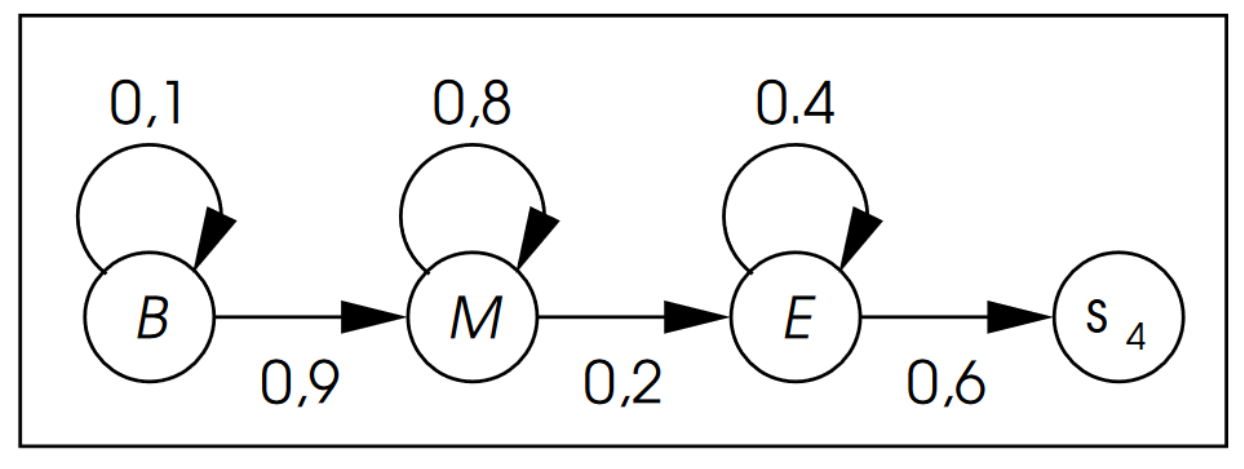
\includegraphics[width=\textwidth]{hmm_voor_t}
			\caption{Het HMM voor het foneem 't'.}
			\label{fig:hmm_voor_t}
		\end{figure}
	
		\item Het HMM voor een woord wordt gevormd door de HMM's voor zijn fonemen aaneen te schakelen. Als een woord $w_i$ de fonemen $f_i$ heeft, dan heeft het HMM 3 $f_i$ staten
		\item Er moet ook nog een model opgebouwd worden om de waarschijnlijkheid van zinnen te modelleren. Dit is echter zeer complex en hierbij wordt er gebruik gemaakt van \textbf{$n$-grammodellen}.
		\begin{itemize}
			\item Een $n$-gram is een sequentie van $n$ woorden.
			\item Als de probabiliteit van alle $n$-grammen gekent is, dan kan dit gebruikt worden om bij $n-1$ woorden het volgende woord te voorspellen.
			\item Een \textbf{unigram} is een $1$-gram dat dan de relatieve frequentie van alle woorden bevat.
			\item Een \textbf{bigram} is een $2$-gram bevat alle mogelijke combinaties van twee opeenvolgende woorden.
		\end{itemize}
	\end{itemize}
	
	

\end{itemize}

\section{Leren van het model}

\chapter{Actieve Systemen}
\begin{itemize}
	\item Klassieke regelbanken worden gebruikt voor expertsystemen, die toelaten om conclusies te trekken uit bepaalde gegevens.
	\item Er kan ook een systeem ontwikkeld worden waar het geheel
\end{itemize}
\section{Eenvoudige systemen}
\begin{itemize}
	\item Bij een eenvoudig systeem is het mogelijk een opsomming te maken van alle visies, acties en hun combinaties.
	\item Bij elke tijdsstap analyseert de actieve eenheid de visie en kiest op basis daarvan een actie. De buitenwereld reageert op deze actie en genereert een nieuwe visie.
	\alert Een visie geeft slechts gedeeltelijke beschrijving van de wereld. Een \textbf{\gls{ac:hmdm}}, wat een uitbreiding is op een \textbf{\gls{ac:hmm}}, tracht dit te modelleren en bestaat uit het volgende:
	\begin{itemize}
		\item Een eindige verzameling van \textbf{staten} $S = \{s_1, ..., s_n\}$. Er is een beginstaat $(s_1)$ en een eindstaat $(s_n)$.
		\item Een eindige verzameling $D = \{d_1, ..., d_l\}$ van \textbf{beslissingen}.
		\item Voor elke $d \in D$ een \textbf{transitiematrix} $T(d)$.
		\item Een \textbf{uitvoeralfabet} $A = \{a_1, ..., a_k\}$. Dit is het alfabet van visies.
		\item Een \textbf{beloningsfunctie} $b: A \rightarrow \mathcal{R}$. Een beloning kan negatief zijn.
		\item Een $n \times k$ \textbf{uitvoermatrix} $U$.
	\end{itemize}
	\item Een \textbf{run} is het hele proces van begintoestand en eindtoestand. 
	\item Een actieve eenheid moet een \textbf{strategie} $\tau$ hebben. Aan elke letter $a$ van het uitvoeralfabet is er dan een beslissing $\tau(a)$.
	\item \underline{Actieve eenheden zonder onzekerheid:} twee voorwaarden
	\begin{enumerate}
		\item \begin{itemize}		
			\item De staat komt overeen met de visie.
			\item Er is een één op één relatie tussen A en S, waarbij $k = n$ en $U$ een diagonaalmatrix waarbij alle diagonaalelementen 1 zijn.
			\item Noteer $\tau(s) = d$ als een strategie $\tau$ die in staat $s$ beslissing $d$ neemt.
			\item Dit zorgt ervoor dat dat de H uit \gls{ac:hmdm} mag wegvallen.
			\end{itemize}
		\item \begin{itemize}
			\item De overgang naar de volgende staat is helemaal gedetermineerd door de beslissing. 
			\item Elke $T(d)_{ij}$ is ofwel 1 ofwel 0. 
			\item De transitie kan uitgedrukt worden als $T(d, s) = s'$ als $d$ leidt tot een overgang naar staat $s'$.
			\item We krijgen een deterministisch systeem waarbij een staat $s$ in één tijdsstap overgaat in de staat $T(\tau(s), s)$.
	\end{itemize}
	\end{enumerate}
	\item \underline{Voorbeeld: figuur \ref{fig:doolhof_exploratie}} 
	\begin{figure}[ht]
		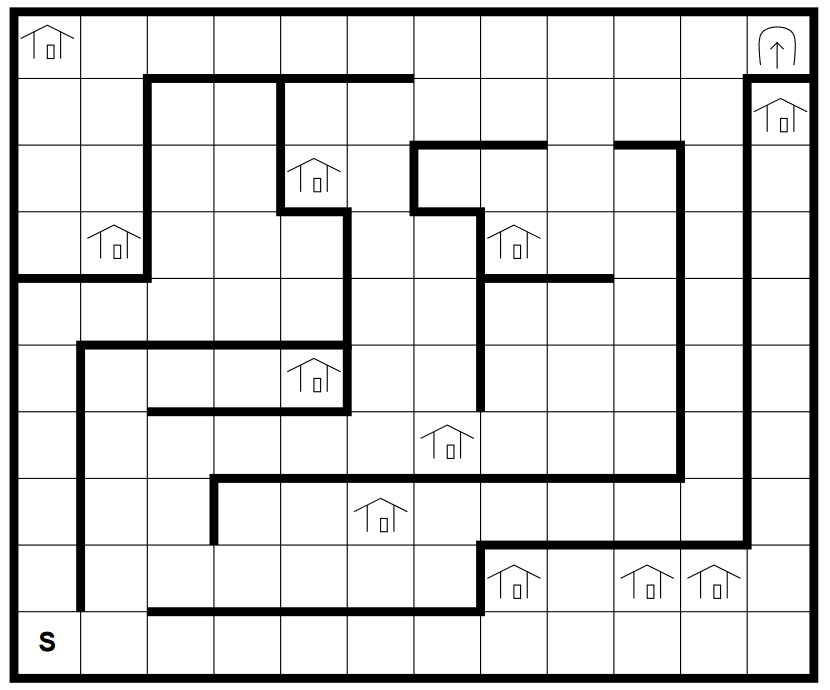
\includegraphics[width=\linewidth]{doolhof_exploratie}
		\caption{Een eenvoudige leerwereld.}
		\label{fig:doolhof_exploratie}
	\end{figure}
	\begin{itemize}
		\item Een doolhof met startpositie $s$.
		\item Op elke plaats kan de eenheid beslissen één vakje verder te gaan in horizontale of verticale richting. De eenheid kan niet door dikke lijnen heen.
		\item Het verplaatsen van een vakje naar een volgend vakje kost 1 dag.
		\item De eenheid kan maar voor 10 dagen verplaatsingen doen.
		\item Een hut kan onbeperkt het aantal dagen terug opvullen tot 10.
		\alert We gaan ervan uit dat er geen lussen zijn in het optimale pad. De eenheid zal dus niet telkens twee hutten oneindig lang blijven bezoeken.
		\item De eenheid moet nu met zoveel mogelijk dagen de uitgang (rechtsboven) weten te bereiken. 
		\item Om een MDM te maken wordt voor elk vakje 11 staten bijgehouden. Bij elke staat wordt de coördinaten van het vakje aangevuld met het aantal dagen van de eenheid bijgehouden.
		\item De beginstaat is dan $((0, 0), 10)$.
		\item Er kan aan elke staat een waarde gegeven worden:
		\begin{itemize}
			\item Voor de eindstaten waar de eenheid sterft is de waarde -10.
			\item Voor de eindstaten aan de uitgang, $((11, 9), i)$ is de waarde $i + 1$.
			\item Voor de andere vakjes is er een verband tussen de waardering voor de staat door eenheid en de gevolgde strategie.
		\end{itemize}
		\item In het algemeen geval wordt de formule gegeven:
		{\color{OliveGreen}	$$\omega_\pi(s) = b(s) + \omega_\pi(T(\pi(s), s))$$}
		\begin{itemize}
			\item De strategie $\pi$ beïnvloedt de waarde $\omega_\pi(s)$ als $\pi$ toegepast wordt op een staat $s$.
		\end{itemize}
		\item Aangezien er geen onzekerheid is kan een optimale strategie $\tau_{opt}$ gevonden worden zodat $\omega_{\tau_{opt}}(s) \geq \omega_\tau(s)$. De beslissing $\tau_{opt}(s)$ leidt dan tot een staat $s'$ die voldoet aan
		{\color{OliveGreen}		
		$$\omega_{\tau_{opt}}(s) = b(s) + \max_{\substack{d \in D}} \omega_{\tau_{opt}}(T(d,s))$$
		}
	\item Het kan zijn dat er meerdere optimale strategieën bestaan. De formule kan dan herschreven worden door het maximum van alle strategieën te pakken, zodat de keuze van strategie niet meer uitmaakt:
		{\color{OliveGreen}		
		$$w^*(s) = b(s) + \max_{\substack{\tau}}\omega_\tau(T(d, s))$$
	}
	Voor elke optimale strategie geldt dat $\omega_{\tau_{opt}}(s) = \omega^*(s) $
	\end{itemize}
\end{itemize}

\subsection{Exploratie zonder onzekerheid}
\begin{itemize}
	\item Een \textbf{exploratiestrategie} laat de eenheid leren door te zien wat er gebeurt.
	\item Een klassieke strategie neemt elke keer dezelfde beslissing voor elke staat.
	\item Een exploratiestrategie $\xi$ kent aan elke combinatie $(s, d)$ een probabiliteit $\xi(s, d)$ toe. Hierbij geldt:
	$$\sum_D \xi(s, d) = 1$$
	\item Als de eenheid in staat $s$ terechtkomt, wordt beslissing $d$ gekozen op basis van de probabiliteit.
	\item De totale opbrengst $W$ kan voor een specifieke run bepaald worden. Voor alle staten die de eenheid gepasseerd is, kan de benaderde schatting $\omega(s)$ van $\omega^*(s)$ vervangen worden door
	$$\max\{W, w(s)\}$$
\end{itemize}

\subsection{Exploratie met onzekerheid}
\begin{itemize}
	\item Hierbij is er geen één op één relatie tussen staat en visie. De overgang naar een nieuwe staat is slechts probabilistisch afhankelijk van de genomen beslissing.
	\item Gegeven een staat $s_i$ en een beslissing $d$, dan is de waarschijnlijkheid om over te gaan naar $s_j$ gelijk aan $T(d)_{ij}$. 
	\begin{itemize}
		\alert Dit heeft als gevolg dat de winst van een strategie $\pi$ niet exact kan voorspeld worden als we uit een staat $s$ vertrekken.
		\item Er kan wel een \textbf{verwachtingswaarde} berekend worden:
		{\color{OliveGreen}
		$$\omega_\pi(s_i) = b(s_i) + \sum_j T(\pi(s_i))_{ij}\omega_\pi(s_j)$$
		}
	\end{itemize}
	\item Een lerende eenheid kent het systeem echter niet. Het moet niet alleen een schatting maken van de waarde van alle staten, maar ook van de overgangswaarschijnlijkheden $T(d)_{ij}$. Stel $A_{ij}$ het totaal aantal keer dat de eenheid in staat $s_j$ is geraakt vanuit staat $s_i$ door $d$ te gebruiken, dan wordt volgende schatting gebruikt:
	$$T(d)_{ij} \approx \frac{A_{ij}}{\sum_{k=1}^{n}A_{ik}}$$
\end{itemize}

\section{Complexe systemen}
\begin{itemize}
	\item Bij eenvoudige systemen is er informatie beschikbaar over elke staat. Bij systemen met onzekerheid moet zelf voor elke combinatie $(s, d)$ de overgangswaarschijnlijkheid naar elke staat bijgehouden worden.
	\alert Niet haalbaar voor een groot aantal staten.
	\item Invoering van \textbf{actieve regelbanken}, deze bevat regels van de vorm
			\begin{equation*}
				\begin{split}
				& \hbox{\textbf{als} premisse} \\
				& \hbox{\textbf{dan} voer actie uit} 
				\end{split}
			\end{equation*}
	\good Eenvoudiger dan klassieke regelbanken: een actie kan geen deel uitmaken van de premisse van een andere regel.
	\item Om de actieve regelbank zo klein mogelijk te houden worden regels zo algemeen mogelijk genomen. In het geval van conflicten zoals
				\begin{equation*}
					\begin{split}
					& \hbox{\textbf{als} } a > 3 \hbox{ en } a \leq 5 \\
					& \hbox{\textbf{dan} voer actie 1 uit} 
					 \\[3ex]
					& \hbox{\textbf{als} } b == 2 \\
					& \hbox{\textbf{dan} voer actie 2 uit} \\
					\end{split}
				\end{equation*}
	wordt meestal de regel gekozen die het minst algemeen is. In sommige gevallen wordt er ook randomisatie gebruikt om variatie te hebben tussen acties.
	\item Actieve regelbanken worden gebruikt bij genetische algoritmen.
\end{itemize}

\section{Genetische algoritmen}
\begin{figure}
	
	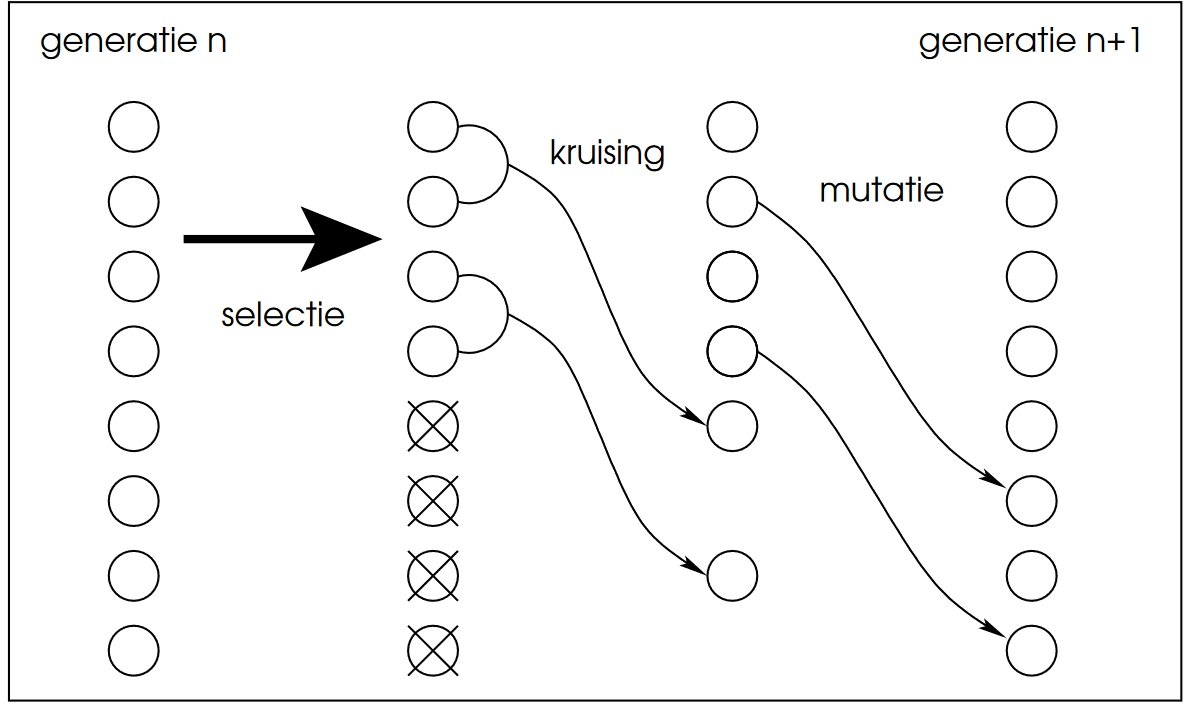
\includegraphics[width=\textwidth]{genetisch_algoritme}
\end{figure}
\begin{itemize}
	\item Start vanuit een grote groep van strategieën, de \textbf{populatie}.
	\item Wijzig nu de populatie door strategieën te verwijderen, toe te voegen of aan te passen zodat uiteindelijk een strategie gevonden is die efficiënt is.
	\item We maken gebruik van \textbf{generaties}. Elke generatie bestaat uit een populatie die even groot is. De volgende generatie wordt bekomen in twee stappen:
	\begin{enumerate}
		\item De populatie wordt uitgedund zodat enkel de beste strategieën overblijven.
		\begin{itemize}
			\item Er moet een \textbf{geschiktheidsfunctie} gedefinieerd worden.
			
		\end{itemize}
		\item Gebaseerd op de overblijvende strategieën wordt de populatie terug aangevuld. Hier kan er kruising of mutatie toegepast worden. 
		\begin{itemize}
			\item Een \textbf{kruising} neemt twee exemplaren uit de populatie en vermengt deze, zodat de nakomeling eigenschappen heeft van de ouders.
			\item Een \textbf{mutatie} voert een kleine wijziging door aan een strategie uit de populatie.
		\end{itemize}
	\end{enumerate}
	\item \underline{Voorbeeld: uurroosterprobleem}
	\begin{itemize}
		\item Er zijn een aantal studentengroepen die elk een aantal cursussen volgen die gegeven worden door bepaalde docenten. Verder zijn er klaslokalen.
		\item Er moet een uurrooster opgemaakt worden dat aan een aantal eisen voldoet. Er zijn twee soorten eisen:
		\begin{enumerate}
			\item \textbf{Harde eisen}: \begin{itemize}
				\item Elke cursus moet gegeven worden.
				\item Een docent kan maar één cursus geven op een moment.
				\item Een studentengroep kan maar les volgen op één moment.
				\item Elke les moet doorgaan in een lokaal dat geschikt is voor de les.
				\item Er kunnen geen twee lessen tegelijk doorgaan in hetzelfde lokaal.
			\end{itemize}
			\item \textbf{Zachte eisen}:
			\begin{itemize}
				\item Er moeten zo weinig mogelijk springuren zijn.
				\item De lokaalwissels moeten beperkt blijven.
				\item enz...
			\end{itemize}
		\end{enumerate}
		\item De beginpopulatie kan nooit aan alle voorwaarden voldoen. Daarom worden onmogelijke uurroosters toegelaten, maar deze krijgen een slechte geschiktheid. 
		\begin{enumerate}
			\item Voor elke harde eis die niet voldaan is worden duizend strafpunten afgetrokken.
			\item Voor elke zachte eis die niet voldaan is wordt één punt afgetrokken.
		\end{enumerate}

	\end{itemize}
\end{itemize}

\section{Optimalisatie van één strategie}
\begin{itemize}
	\item Elke regel krijgt een waardering $\omega(r)$, die aangeeft wat de verwachte winst is wanneer $r$ toegepast wordt, als ervan uitgegaan wordt dat voor de rest van de oplossing dezelfde strategie gebruikt wordt.
	\item Een regel die uitgevoerd wordt kan ook de waarde van andere regels wijzigen.
	\item Het \textbf{leerproces}:
	\begin{itemize}
		\item Normaal gezien zijn overlappende regels slecht, maar hier zijn ze nuttig:
		\begin{itemize}
			\item Als er twee regels zijn met dezelfde premise maar andere actie, wordt diegene bijgehouden die de hoogste waardering oplevert.
			\item Als er twee regels zijn met verschillende premissen maar dezelfde acties, waarbij premisse 1 meer algemeen is dan premisse 2, dan behouden we premisse 1 als er visies zien waarbij de tweede regel niet van toepassing is, anders premisse 2.
		\end{itemize}
		\item Twee fasen:
		\begin{enumerate}
			\item De \textbf{exploratiefase}:
			\begin{itemize}
				\item Er is een \textbf{regelverzameling} $A(v)$ van een visie. 
				\item Dit is de verzameling regels waarvan de premisse beantwoord aan $v$.
				\item Als we in visie $v$ zitten nemen we een regel uit $A(v)$, en voeren de daarbijhorende actie $\alpha$ uit. De regel kan gekozen worden door bijvoorbeeld een random keuze te maken met de waarderingen van de regels als gewicht.
				\item De actie $\alpha$ zorgt voor een nieuwe visie $v'$.
				\item Om na te gaan hoe goed deze actie is, moet er een waarde toegekend worden aan $v'$.
				$$\omega(v') = b(v') + \max_{r \in A(v')} \omega(r)$$
				\item De verzameling $A(v)$ wordt in twee delen opgesplitst:
				\begin{enumerate}
					\item[1. ] Elke regel $r$ in $A(v)$ die als actie $a$ voorstelt, kan de waardering $\omega(r)$ door onzekerheid aangepast worden met een vergeetfactor $\alpha, 0 < \alpha < 1$:
					$$\omega(r) \rightarrow (1 - \alpha)\omega(r) + \alpha\omega(v')$$
					\item[2. ] Voor elke andere regel $r$ in $A(v)$ die een andere actie al $a$ voorstelt, vermindert de waardering met een vergeetfactor $\beta$ die kleiner is dan $\alpha$:
					$$\omega(r) \rightarrow (1 - \beta)\omega(r)$$
				\end{enumerate}
			\end{itemize}

			\item De \textbf{regelaanpassingsfase}:
			\begin{itemize}
				\item Regels met een lage waardering worden verwijderd, vaak door ze te veranderen.
				\item Er kan bijgehouden worden hoe vaak regels gebruikt werden in de exploratiefase. Deze hebben minder kans om verwijderd te worden.
				\item Als een regel soms heel goed en soms heel slecht presteert, dan kan de regel \textbf{gesplitst} worden:
				\regel{$3 \leq x \leq 5$}{Actie A}
				Er kan een variabele ingevoerd die tracht het goede en het slechte deel te scheiden:
				\regel{$3 \leq x \leq 5$ en $y < 10$}{Actie A}
				\regel{$3 \leq x \leq 5$ en $y > 10$}{Actie A}
				\item Regels kunnen ook \textbf{samengevoegd} worden. Als twee regels dezelfde actie voorstellen, en een grote overlapping hebben kan dit nuttig zijn.
				\item De premissen van regels die goed presteren kunnen ook verruimd worden.
			\end{itemize}
		\end{enumerate}
	\end{itemize}
\end{itemize}
\section{Combinaties}


\chapter{Neurale netten}
\begin{itemize}
	\item Een neural netwerk is een informatieverwerkend geheel dat de vorm heeft van een \textbf{gewogen gerichte graaf}.
	\item De knopen van deze graaf worden \textbf{neuronen} genoemd.
	\item Deze knopen sturen signalen naar alle verdere knopen in de graaf met een sterkte die afhangt van de som van de invoersignalen.
	\item De gewichten van de takken van de graaf geven aan hoeveel het signaal dat langs die tak loopt versterkt wordt.
\end{itemize}


\section{Vergelijking met computers}
\begin{itemize}
	\item Bij een \textbf{computer}:
	\begin{enumerate}
		\item Men moet de machine tot op het laatste detail vertellen wat het algoritme is om de invoer te verwerken. Dit houdt automatisch in dat er iemand moet geweest zijn dat die algoritme kende.
		\item De computer is zeer gevoelig voor onverwachte invoer: een fout in de invoer kan enkel herstelt worden als het algoritme op deze fout voorzien is.
		\item De kleinste fout in apparatuur kan ertoe leiden dat de uitvoer corrupt wordt. 
		\item Elk begrip en object van de verwerking is duidelijk localiseerbaar in het geheugen.
	\end{enumerate}
	\item Bij een \textbf{neuraal net}:
	\begin{enumerate}
		\item Een neuraal netwerk wordt niet geprogrammeerd meer leert.
		\item Een neuraal netwerk is zeer goed in veralgemenen: het kan invoer verwerken die lijkt op de al geziene invoer.
		\item Een neuraal netwerk is ongevoelig voor beschadigingen.
		\item Objecten zijn niet localiseerbaar.
	\end{enumerate}
	\item Twee manieren om kunstmatige neurale netwerken te maken:
	\begin{enumerate}
		\item \textbf{Hardwarematig}: er worden elektronische componenten geconstrueerd die dezelfde functies hebben als een natuurlijk neuron. 
		\item \textbf{Softwarematig}: de werking van een neuraal netwerk wordt gesimuleerd met een programma.
	\end{enumerate}
\end{itemize}
\section{De biologische grondslagen}
\begin{itemize}
	\item Zenuwstelsel bestaat uit zenuwcellen (neuronen).
	\item Er zijn drie soorten neuronen:
	\begin{enumerate}
		\item \textbf{Invoerneuronen}: Deze zetten de signalen van de buitenwereld om in signalen die verwerkt kunnen worden door andere neuronen.
		\item \textbf{Interneuronen}: Deze verwerken de informatie.
		\item \textbf{Uitvoerneuronen}: Deze geven informatie door aan de buitenwereld.
	\end{enumerate}
	\item Structuur van een interne neuron:
	\begin{itemize}
		\item De \textbf{soma} is het centrale deel.
		\item De \textbf{dendrieten} zijn vertakkingen die vertrekken uit de soma.
		\item De \textbf{axon} is een lange, enkelvoudige, vertakking die ook vertrekt uit de soma.
		\begin{itemize}
			\item Uit de axon kunnen andere vertakkingen zich voordoen.
			\item Elke vertakking eindigt met een synaps, die de vertakking verbindt met de dendriet van een ander neuron.
		\end{itemize}
	\end{itemize}
	\item Structuur van een invoerneuron:
	\begin{itemize}
		\item Idem interne neuron maar zonder dendrieten.
	\end{itemize}
	\item Structuur van een uitvoerneuron:
	\begin{itemize}
		\item Idem interne neuron maar de axon is vervangen met een specifieke verbinding voor de functie van die zenuwcel.
	\end{itemize}
	\item De puls is een elektronische stroomstoot. Deze loopt doorheen de axon en komt aan bij alle synapsen van dit axon.
	\item Er zijn twee situaties wanneer een neuron een puls kan afvuren:
	\begin{enumerate}
		\item Een \textbf{excitatorische} of \textbf{prikkelende} puls ?? 
		\item Een \textbf{inhibitorische} of \textbf{remmende} puls ??
	\end{enumerate}

\end{itemize}
\chapter{Kunstmatige Netwerken}
Enkele notaties:
\begin{itemize}
    \item De neuronen van het netwerk worden aangeduid met de letters $x$, $y$ of $z$. Deze worden genummerd door een onderindex $i$.
    \item De verbindingen in de graaf krijgen geen apart symbool. Het gewicht van de tak die van $x_i$ naar $x_j$ gaat noteren we als $w_{ij}$; in het geval dat er geen verbinding is, is $w_{ij} = 0$.
    \item De uitvoer van neuron $x_i$ duiden we aan met $u_{i}$.
    \item Een rij getallen die een vector voorstellen worden geschreven met een vette letter: $\textbf{v} = (v_1, ... v_n)$. 
\end{itemize}
\begin{figure}[ht]
    \centering
    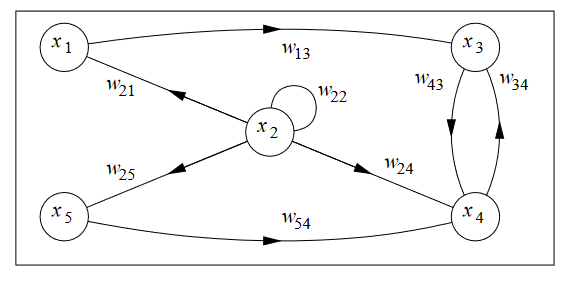
\includegraphics[width=\textwidth]{neuraal_net}
    \caption{Schema van een neuraal net.}
    \label{}
\end{figure}

Een neuraal net is vaak ingedeeld in verschillende lagen, waarin elke laag een verschillende functie heeft. De nulde laag bestaat uit de invoercellen. Er zijn twee vormen:
\begin{enumerate}
    \item \textbf{Gesloten gelaagde netten}: Er zijn enkel verbindingen mogelijk tussen opeenvolgende lagen van het net. Van laag $k$ naar $k + 1$, of met terugkoppeling, van $k + 1$ naar $k$.
    \begin{figure}[ht]
        \centering
        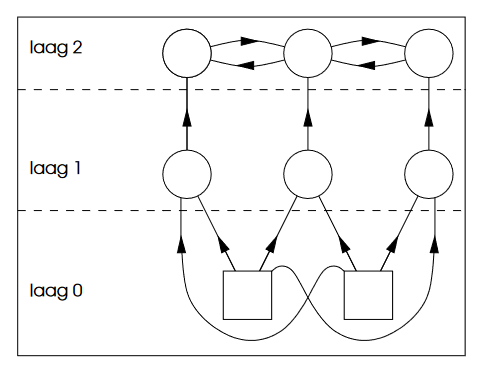
\includegraphics[width=0.5\textwidth]{gesloten_gelaagd_net}
        \caption{Gesloten gelaagd net}
        \label{}
    \end{figure}
    \item \textbf{Open gelaagde netten}: Er zijn verbindingen mogelijk tussen twee willekeurige lagen.
    \begin{figure}[ht]
        \centering
        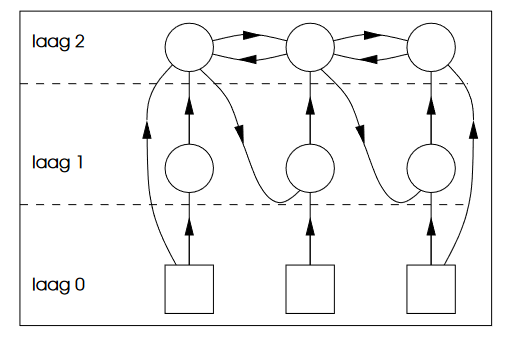
\includegraphics[width=0.5\textwidth]{open_gelaagd_net}
        \caption{Open gelaagd net}
        \label{}
    \end{figure}
\end{enumerate}

\section{Artificiële neuronen}
Er zijn drie belangrijke kenmerken die kunstmatige neuronen kunnen onderscheiden:
\begin{enumerate}
    \item De \textbf{reactiefunctie}: deze geeft aan wat de uitvoer is in functie van de invoer.
    \item De \textbf{uitvoeringsmethode}: beschrijft hoe de verandering in uitvoer wordt doorgevoerd. Twee opties:
    \begin{enumerate}
        \item Direct.
        \item Wachten op een extern signaal (bv. Hopfieldnetten).
    \end{enumerate}
    \item De \textbf{tijd}: vaak wordt er verondersteld dat alle wijzigingen ogenblikkelijk gebeuren.
\end{enumerate}

\section{TLU's}
TLU = Threshold Logic Unit

\begin{itemize}
    \item Wordt gebruikt in binaire netwerken.
    \item De werking van een neuron wordt bepaald door een drempelwaarde, die voor elke neuron verschillend kan zijn.
    \item Als de drempelwaarde van neuron $x_i$ gelijk is aan $T_i$, wordt de uitvoer gegeven door
    $$u_i = \begin{cases}
        1 \quad \hbox{als}\quad \sum_jw_{ji}u_j \geq T_i \\
        0 \quad \hbox{als}\quad \sum_jw_{ji}u_j < T_i
    \end{cases}$$
    \alert Ook mogelijk om extra neuron $x_0$ in te voeren, die verbonden is met elke andere neuron met gewicht $w_{0i} = -T_i$. Op die manier wordt de reactiefunctie gelijk voor alle neuronen:
    $$f(r) = \begin{cases}
        1 \quad \hbox{als}\quad r \geq 0 \\
        0 \quad \hbox{als}\quad r < 0
    \end{cases}$$
\end{itemize}

\section{Analoge netten}
\begin{itemize}
    \item Leunt meer aan met biologische netwerken.
    \item De uitvoer van een analoog neuron kan continu veranderen: als de invoer van het neuron vergroot, vergroot ook zijn uitvoer.
    \item De uitvoer is wel begrensd
    \item Vaak wordt stijgende functie gebruikt:
    $$\sigma(r) = \frac{1}{1 + \exp(\frac{-r}{R})}$$
    Voor $R \rightarrow 0$ is deze functie bijna binair. 

    Voor $R \rightarrow \inf$ verloopt de functie vlakker.
    \item Andere functies met analoge eigenschappen: boogtangens.
\end{itemize}

\section{Tijd}

\section{Leren}
\chapter{Informatieverwerking met neurale netten}
Drie vormen die zullen toegepast worden op TLU's:
\begin{itemize}
    \item Via binaire functies.
    \item Via automaten.
    \item Via associatieve geheugens (Hopfieldnet).
\end{itemize}

Belangrijk nadeel aan TLU: het geeft geen realistisch model van de manier waarop het netwerk leert.

\section{Binaire functies}
\begin{itemize}
    \item Alle binaire functies kunnen gerealiseerd worden met een tweelagig net van TLU's (Stelling van McCulloch en Pitts).
    \item Stel een aantal elementaire logische uitspraken $v_1, ... v_n$.
    \item Hier kunnen complexe uitdrukkingen mee gevormd worden: $\neg v_1 \wedge (v_2 \vee v_3) \Rightarrow (v_1 \Rightarrow \neg v_3)$
    \item Neuraal net opstellen om na te gaan of de uitspraak waar is of niet.
    \begin{itemize}
        \item Het netwerk bestaat uit TLU's die de waarden $v_i$ als invoer krijgen in de vorm van $0$ of $1$.
        \item Als de stelling waar is geeft TLU $1$ terug, anders $0$.
    \end{itemize}
    \item Een binaire functie is een functie $F$ van de verzameling binaire getallen met $n$ cijfers, $\{0, 1\}^n$ naar deze van binaire getallen met $k$ cijfers $\{0, 1\}^k$, waarbij $n$ en $k$ vooraf positief gehele getallen zijn. 
    \item Een neuraal net heeft dan $n$ ingangen en $k$ uitgangen.
    \item Als de invoer aan het net gegeven wordt, wachten we tot alle neuronen een stabiele toestand bereiken, en zo is de uitvoer alleen afhankelijk van de invoer. 
    \item Een net realiseert een binaire functie $F$ als de uitvoer beschreven wordt als functie van de invoer. 
    \item Gegeven een binaire functie $F$, kan er een net gevonden worden die deze functie realiseert?
    \begin{itemize}
        \item We moeten alleen kijken naar $k = 1$ want als $k > 1$, dan kunnen $k$ netwerken gekozen worden met 1 uitvoercomponent. Elk van deze netwerken zorgt dan voor 1 component van $F$.
        \begin{itemize}
            \item Stel $n = k = 2, F : \{0, 1\}^2 \rightarrow \{0, 1\}^2, F_1 : \{0, 1\} \rightarrow \{0, 1\}^2, F_2 : \{0, 1\}^2 \rightarrow \{0, 1\}$

            \begin{align*}
                F(0, 0) = (0, 1) \quad F_1(0, 0) = 0 \quad F_2(0, 0) = 1 \\
                F(0, 1) = (1, 1) \quad F_1(0, 1) = 1 \quad F_2(0, 1) = 1 \\
                F(1, 0) = (1, 1) \quad F_1(1, 0) = 1 \quad F_2(1, 0) = 1 \\
                F(1, 1) = (0, 0) \quad F_1(1, 1) = 0 \quad F_2(1, 1) = 0 \\
            \end{align*}
            \item Samenvoegen van $F_1$ en $F_2$ geeft $F$.
        \end{itemize}
        \item Stel binaire functie $F$ met invoer $(b_1, ..,. b_n)$ en uitvoer $F(b_1, ..., b_n)$.
        \item Het net dat we zoeken heeft $n$ invoerneuronen en $k$ uitvoerneuronen. 
        \item De laag van invoerneuronen (nulde laag) vormt geen deel van het neuraal net.
        \item Dus een tweelagig net bevat de invoerneuronen, de uitvoerneuronen en nog één laag van tussenliggende neuronen.
        \item Functies die met een éénlagig net kunnen gerealiseerd worden:
        \begin{enumerate}
            \item De \textbf{OF}-functie, die (0, ..., 0) op 0 afbeeldt, en alle andere combinaties op 1 $ \rightarrow$ neuron met $n$ ingangen en $T = 0.5$.
            \item De \textbf{select}-functie die een vooropgegeven bitcombinatie $(b_1, ..., b_n)$ op 1 afbeeldt, en alle andere op 0 $\rightarrow$ neuron met $n$ ingangen en $w_i = 2b_i - 1$.
        \end{enumerate}
        \item \textbf{Stelling: (McCulloh en Pitts)} Zij $F : \{0, 1\}^n \rightarrow \{0, 1\}^k$ een willekeurige binaire functie. Dan is er een gesloten gelaagd netwerk met ten hoogste twee lagen dat $F$ weergeeft. Anderzijds bestaan er functies die niet door een netwerk met één laag kunnen worden weergegeven.
        \begin{itemize}
            \item Als $F$ $\ell$ bitcombinaties op $1$ afbeeldt:
            \begin{enumerate}
                \item De eerste laag bevat $\ell$ neuronen. Elk daarvan realiseert de selectiefunctie voor een bitcombinatie die op $1$ moet worden afgebeeld.
                \item De tweede laag bestaat uit een neuron met $\ell$ ingangen die de OF-functie realiseert.
            \end{enumerate}
        \end{itemize}
    \end{itemize}
\end{itemize}


\section{Automaten}
\begin{itemize}
    \item De Mooreautomaat heeft volgende kenmerken:
    \begin{itemize}
        \item Een eindige verzameling staten $Q = \{q_1, ..., q_{|Q|}\}$.
        \item Een invoeralfabet $S = \{s_1, ..., s_{|S}\}$.
        \item Een uitvoeralfabet $G = \{g_1, ..., g_{|G|}\}$.
        \item Een transitiefunctie $d : Q \times S \rightarrow Q$.
        \item Een uitvoerfunctie $\ell : Q \rightarrow g$.
        \item Een beginstaat $q_I \in Q$.
    \end{itemize}
    \item Aangezien we met TLU's werken is 
    $$S \subset \{0, 1\}^n \qquad G \subset \{0, 1\}^k$$
    \item Het is tijdsafhankelijk: de uitvoer van een neuron op tijdstip $t$ hangt af van de totale invoer op tijdstip $t - 1$. 
    \item De invoer wordt aangevoerd op even tijdstippen, $t = 0, 2, 4, ...$. De oneven tijdstippen geeft de automaat de kans om de invoer te verwerken.
    \item Twee veronderstellingen:
    \begin{enumerate}
        \item Het invoeralfabet is exact de verzameling van binaire strings van lengte $n$ bestaande uit $n - 1$ nullen en één 1.
        \item Het invoeralfabet is exact de verzameling van binaire strings van lengte $k$ bestaande uit $n - 1$ nullen en één 1.
    \end{enumerate}
\end{itemize}


\chapter{Het Classificatieprobleem}

\begin{itemize}
    \item Slechts 2 klassen
    \begin{itemize}
        \item Geen probleem indien meerdere klassen: ze kunnen beschouwd worden als een combinatie van tweeklassenproblemen.
        \item Stel drie klassen $A$, $B$ en $C$: los eerst classificatieprobleem op met $A$ en niet$-A$, en daarna voor $niet-A$ het probleem $B$ en $C$ op te lossen.
    \end{itemize}
    \item Een neuron deelt de $n$-dimensionale ruimte op in twee stukken, die men halfruimten noemnt.
    \item De scheiding tussen deze twee halfruimten is een verzameling van de vorm:
    $$\{\textbf{x} : \textbf{x} \cdot \textbf{w} - T = 0\}$$
\end{itemize}

\section{Harde classificatie}
\begin{itemize}
    \item Stel $\mathcal{L}$ de leerverzameling.
    \item Deze is verdeeld in twee klassen $\mathcal{L}^+$ en $\mathcal{L}^-$.
    \item $\mathcal{L}$ is lineair scheidbaar als er een halfruimte bestaat die alle punten van $L^+$ bevat, en geen enkele van $L^-$, terwijl er ook geen punten op de rand mogen liggen. 
    $$\textbf{x} \cdot \textbf{w} = \begin{cases}
        > T \quad \hbox{als} \quad \textbf{X} \in \mathcal{L}^+ \\
        < T \quad \hbox{als} \quad \textbf{X} \in \mathcal{L}^-
    \end{cases}$$
    \item Dit komt overeen met het bestaan van een neuron met $n$ invoerkanalen, elk met gewicht $w_i$, en met een drempel $T$ zodanig dat de invoer strikt positief is voor een punt uit $\mathcal{L}^+$ en strikt negatief voor een punt uit $\mathcal{L}^-$.
    \item Neem een polaire TLU, dan is de uitvoer +1 voor elementen uit $\mathcal{L}^+$ en -1 voor elementen uit $\mathcal{L}^-$. Dit is de eenvoudigste vorm van het \textbf{perceptron}.
    \item Hoe moeten de gewichten gekozen worden?
    \begin{itemize}
        \item Om berekeningen te vergemakkelijken wordt de drempel $T$ weggewerkt door een extra dimensie toe te voegen, waarbij elk component in die dimensie altijd de waarde 1 bevat en zodat $T = -\omega_0$.
        \item We zoeken nu een vector in $\mathcal{R}^{n + 1}$ zodanig dat
        $$\textbf{x} \cdot \textbf{w} > 0 \; \hbox{als}\;\textbf{x} \in \mathcal{L}^+ \qquad \textbf{-x} \cdot \textbf{w} > 0 \; \hbox{als}\;\textbf{x} \in \mathcal{L}^-$$
        \item Vervang $\mathcal{L}$ door $\mathcal{P}$
        $$\mathcal{P}_i = \begin{cases}
            \textbf{x} \; & \hbox{als}  \;\textbf{x} \in \mathcal{L}_i^+ \\
            \textbf{-x} \; & \hbox{als}  \;\textbf{x} \in \mathcal{L}_i^-
        \end{cases}$$
        \item Als we een vector \textbf{x} uit $\mathcal{P}$ aanbieden aan perceptron, dan moet deze $1$ als uitvoer hebben. 
        \item Algoritme:
        \begin{enumerate}
            \item Initialiseer de gewichten op 0
            \item Zolang (geen foutlees parcours en niet te veel pogingen)
   
                \item Voor elke vector \textbf{x} uit $\mathcal{P}$
                \begin{enumerate}
                    \item Als $\textbf{x} \cdot \textbf{w} \leq 0$
                    \item Vervang $\textbf{w}$ door $\textbf{w} + \textbf{x}$
                \end{enumerate}       
        \end{enumerate}
        \item Eindigt dit algoritme?
        \begin{itemize}
            \alert Als we $\textbf{w}$ vervangen door $\textbf{w + x}$ kan het zijn dat $\textbf{x} \cdot (\textbf{w + x})$ nog altijd negatief is.
            \alert Het kan zijn dat een vector $\textbf{v}$ uit $\mathcal{P}$, die al correct geklasseerd was, $\textbf{v \cdot x} > 0$ ,nu verkeerd wordt geklasseerd. Het zou kunnen dat $\textbf{x \cdot v} < 0$ en dan is $\textbf{v} \cdot (\textbf{w + x}) < \textbf{v \cdot w}$.
            \item \textbf{Stelling} Als $\mathcal{L}$ lineair scheidbaar is en $\mathcal{P}$ een eindige verzameling, dan zal het algoritme na een eindig aantal stappen een $\textbf{w}$ vinden die het probleem oplost, en dus $\textbf{x} \cdot \textbf{w} > 0$ voor alle $\textbf{x}$ in $\mathcal{P}$.
            \item Bewijs:
            \begin{itemize}
                \item Stel alle gewichten op 0, en nummer het aantal keer dat een verkeerd geklasseerde vector is tegengekomen.
                \item De vector bij de $k-$de keer hoort noemen we $\textbf{x}(k)$.
                \item De gewichtenvector waarmee we beginnen is $\textbf{w}(0)$, die na de $k-$de keer $\textbf{w}(k)$.
                \item Ons algoritme stelt $\textbf{w}(k) = \textbf{w}(k - 1) + \textbf{x}(k)$ als $\textbf{x}(k) \cdot \textbf{w}(k - 1) \leq 0$
                \item De bovengrens wordt dan:
                \begin{align*}
                    ||\textbf{w}(k)||^2 & = \textbf{w}(k) \cdot \textbf{w}(k) \\
                                        & = (\textbf{w}(k - 1) + \textbf{x}(k)) \cdot (\textbf{w}(k - 1) + \textbf{x}(k)) \\
                                        & = \textbf{w}(k - 1)\cdot \textbf{w}(k - 1) + 2\textbf{w}(k - 1)\cdot\textbf{x}(k) + \textbf{x}(k)\cdot \textbf{x}(k) \\
                                        & = ||\textbf{w}(k - 1)||^2 + ||\textbf{x}(k)||^2 \\
                                        & = ||\textbf{x}(1)||^2 + ... ||\textbf{x}(k)||^2
                \end{align*}
                \item De term $2\textbf{w}(k - 1)\cdot\textbf{x}(k)$ mag verwaarloosd worden, aangezien deze kleiner is dan nul en dus de bovengrens zeker niet zal beïnvloeden.
                \item Er is nu een vector $\textbf{y}$ in $\mathcal{P}$ met de grootste norm, $||\textbf{y}||^2 = M$ en $||\textbf{x}||^2 \leq M$ voor alle andere $\textbf{x}$ in $\mathcal{P}$. Hieruit volgt
                $$||\textbf{w}(k)||^2 \leq kM$$
                \item ...
            \end{itemize}
        \end{itemize}
        
    \end{itemize}
    \alert We weten niet of ons probleem lineair scheidbaar is.
    \good Wel weten we dat voor een leerverzameling $\mathcal{L}$ waarbij $\mathcal{L}^+$ en $\mathcal{L}^-$ geen gemeenschappelijke elementen hebben, dat er een drielagig net kan geconstrueerd worden dat een scheiding van $\mathcal{L}$ kan uitvoeren.
\end{itemize}


\section{Zachte classificatie}


\section{De deltaregel}
\begin{itemize}
    \item Twee versies:
    \begin{enumerate}
        \item \begin{itemize}
            \item Analoog netwerk, dat bestaat uit één neuron.
            \item Leerverzameling $\mathcal{L}$ die bestaat uit meetvectoren $\textbf{v}$ en gewenste uitvoer $y(\textbf{v}) \in [-1, +1]$ waarbij $y$ strikt stijgend is en overal een afgeleide heeft, en dat deze afgeleide verschilt van nul.
            \item Bijvoorbeeld tangens hyperbolicus:
            $$f(r) = \frac{e^{r} - e^{-r}}{e^r + e^{-r}}$$
            \item De afgeleide is:
            $$f'(r) = 1 - (f(r))^2$$
            \item Veronderstel een meetvector $\textbf{v}$, en een resultaat $u$ die verschilt van $y(\textbf{v})$.
            \item De uitvoerfout is hier $e = y(\textbf{v}) - u$.
            \item De fout op de invoer van het neuron:
            \begin{itemize}
                \item De invoer van het neuron is $a = \sum_i(w_iv_i)$ en $f(a) = u$.
                \item Voor kleine waarden van $\delta$ geldt:
                $$f(a + \delta) \approx f(a) + \delta f'(a)$$
                \item Neem $\delta = e/f'(a)$, dan is $f(a + \delta) \approx y(\textbf{v})$.
                \item Vervang elke $\textbf{w}$ door $\textbf{w} + \Delta \textbf{w}$ zodat:
                \begin{itemize}
                    \item De nieuwe invoer van het neuron gelijk is aan $a + \delta$.
                    \item De wijziging zo klein mogelijk is, $||\Delta \textbf{w}||$ is minimaal.
                \end{itemize}
                \item Hier volgt $(\textbf{w} + \Delta \textbf{w}) \cdot \textbf{v} = a + \delta$.
                \item Schrijf $\Delta \textbf{w}$ als
                $$\Delta \textbf{w} = A\textbf{v} + \textbf{y}$$
                met $\textbf{y}$ loodrecht op $\textbf{v}$ en (als gevolg) $A = \frac{\delta}{||\textbf{v}||^2}$ 
                \item $\textbf{y}$ moet gekozen worden zodanig dat $\Delta \textbf{w}$ minimaal is, en dat is bij $\textbf{y} = 0$.
                \item De (eerste versie) deltaregel van een neuron is:
                $$\Delta \textbf{w} = \frac{y(\textbf{v}) - u}{f'(a)||\textbf{v}||^2}\textbf{v}$$
            \end{itemize}
        \end{itemize}
        \begin{itemize}
            \item Gegeven een invoervector $\textbf{v}$.
            \item Stel een kleine wijziging $\tau$ voor gewicht $w_i$.
            \item Hoe wijzigt $u$, de uitvoer van het netwerk?
            \item De invoer verandert: $a = a + \tau v_i$.
            \item De uitvoer verandert: $f(a + \tau v_i) \approx f(a) + \tau v_i f'(a)$.
            \item De factor $v_i f'(a)$ is de partiële afgeleide van $u$ naar $w_i$, die genoteerd wordt als $\partial_{w_i}i$.
    
            $$\partial_{\textbf{w}}u = (\partial_{w_{0}}u, ..., \partial_{w_{n}}u)$$
            \item Hierbij is $\partial_{\textbf{w}}u = f'(a)\textbf{v}$
            \item De (tweede versie) deltaregel van een neuron is:
            $$\Delta \textbf{w} = \frac{y(\textbf{v}) - u}{||\partial_{\textbf{w}}u||^2}\partial_{\textbf{w}}u$$
            \good Kan ook werken om een meerlagig net zonder terugkoppeling te laten leren.
            \item Eventueel een leerfactor $A$ toevoegen, om al te grote schommelingen te vermijden.
        \end{itemize}

    \end{enumerate}
\end{itemize}
\chapter{Steunvectoren}
\begin{itemize}
    \item Andere aanpak voor harde classificatie voor lineaire en niet-lineaire problemen.
    \item Soms is er ruis en is het onbepaald hoeveel neuronen er nodig zijn.
    \item Hier zien we SVM's (Support Vector Machine) die de vorm hebben van een stemmachine.
\end{itemize}
\section{Basisprincipes}
\begin{itemize}
    \item Terug een leerverzameling $\mathcal{L} = \mathcal{L}^+ \cup \mathcal{L}^-$, of
    $\mathcal{L} = \{\textbf{x_1}, ..., \textbf{x_n}\}$
    \item Een stemmachine heeft een gelijkaardigheidsfunctie $g$.
    \begin{itemize}
        \item Geeft aan hoe goed twee items op elkaar lijken.
        \item Voor gegeven $\textbf{x}$ en variërende $\textbf{z}$ heeft $g(\textbf{x}, \textbf{z})$ de grootst mogelijke waarde voor $\textbf{x} = \textbf{z}$ en neemt de waarde af naarmate $\textbf{z}$ minder op $\textbf{x}$ begint te lijken.
        \item Bijvoorbeeld:
        $$g(\textbf{x}, \textbf{z}) = - ||\textbf{x} - \textbf{z} ||^2$$
        waarbij $g(\textbf{x}, \textbf{z}) = g(\textbf{z}, \textbf{x})$
    \end{itemize}
    \item Basisidee: Vectoren die meer lijken op vectoren uit $\mathcal{L}^+$ worden positief geklasseerd. Vectoren die meer lijken op vectoren uit $\mathcal{L}^-$ worden negatief geklasseerd.
    \begin{enumerate}
        \item (Leerfase)
        
        Elke klasse geeft aan elk van zijn vectoren in $\mathcal{L}$ een gewicht dat aangeeft hoe belangrijk de vector voor de klasse is. De som van de gewichten moet gelijk zijn aan $1$ en de gewichten mogen niet negatief zijn. Ook moet een drempelwaarde $T$ bepaald worden.
        \item (Gebruiksfase)
        \begin{enumerate}
            \item Voor een onbekende vector $\textbf{z}$ zendt elke vector $\textbf{x}_i$ in $\mathcal{L}$ een signaal uit dat aangeeft hoe sterk $\textbf{z}$ op $\textbf{x}$ lijkt.
            \item De klasse telt deze signalen voor zijn klasse op, rekening houdend met de gewichten.
            \item $\textbf{z}$ wordt toegewezen aan de klasse met het sterkste signaal.
        \end{enumerate}
    \end{enumerate}
    \item We kunnen elk element $\textbf{x}$ uit $\mathcal{L}$ beschouwen als een invoerneuron dat, gegeven een item $\textbf{z}$, een signaal uitstuurt hoe goed $\textbf{z}$ lijkt op $\textbf{x}$.
    \item Beide klassen hebben een neuron dat de outputs van alle invoerneuronen voor die klasse verzamelt. Ze kunnen beschreven worden door de reactiefunctie $f(r) = r$.
    \item De gewichten zijn $\alpha_1, ..., \alpha_n$, zodat de totale uitvoer van het uitvoerneuron kan beschreven worden als:
    $$a(\textbf{z}) = \sum_{i = 1}^{n}\alpha_iy_ig(\textbf{x}_i, \textbf{z})$$
    Hierbij is $y_i = 1$ als $\textbf{x} \in \mathcal{L}^+$ en  $y_i = -1$ als $\textbf{x} \in \mathcal{L}^-$
    \item $\textbf{z}$ wordt bij $\mathcal{L}^+$ geklasseerd als $a(\textbf{z}) \geq T$, en anders bij $\mathcal{L}^-$ als $a(\textbf{z}) < T$
    \item De vectoren $\textbf{x}_i$ waarvoor $\alpha_i \neq 0$ worden de steunvectoren genoemd.
    \item Hoe worden de gewichten $\alpha_i$ en de drempelwaarde $T$ bepaald?
    \begin{itemize}
        \item Twee grootheden belangrijk:
        $$m^+ = \min_{y_1=1} a(\textbf{x}_i) \qquad m^- = \min_{y_1=-1} a(\textbf{x}_i)$$
        \begin{enumerate}
            \item De $\alpha_i$ horend bij $\mathcal{L}^+$ worden zo gekozen dat $m^+$ zo groot mogelijk is.
            \item De $\alpha_i$ horend bij $\mathcal{L}^-$ worden zo gekozen dat $m^-$ zo klein mogelijk is.
            \item De drempelwaarde wordt vastgelegd op $\frac{m^+ + m^-}{2}$
        \end{enumerate}
        \item Om regel (1) en (2) optimaal te houden, kan de energiefunctie gebruikt worden:
        $$\mathcal{F}(\alpha_1, ..., \alpha_n) = \frac{1}{2}\sum_{i = 1}^{n}\sum_{j = 1}^{n} \alpha_i\alpha_jy_iy_jg(\textbf{x}_i, \textbf{x}_j)$$
        \item Deze zal altijd minimaal zijn voor $\alpha_1, ..., \alpha_n$ die een oplossing van ons probleem opleveren.
        \item \underline{Bewijs:}
        \begin{itemize}
            \item Beschouw de $\alpha$s die gehecht zijn aan een vector in $\mathcal{L}$ en neem $k$ vast waarbij $y_k = 1$. 
            $$\mathcal{F}(\alpha_1, ..., \alpha_n) = \alpha_k\bigg(\sum_{i \neq k}^n \alpha_iy_ig(\textbf{x}_i, \textbf{x}_k)\bigg) + \frac{1}{2}\alpha^2_kg(\textbf{x}_k, \textbf{x}_k)$$
            \item Neem de afgeleide van $\mathcal{F}$ ten opzichte van $\alpha_k$:
            \begin{align*}
                \partial_{\alpha_{k}}\mathcal{F} & = \bigg(\sum_{i \neq k}^n \alpha_iy_ig(\textbf{x}_i, \textbf{x}_k)\bigg) + \alpha_kg(\textbf{x}_k, \textbf{x}_k) \\
                & = \sum_{i}^n\alpha_iy_ig(\textbf{x}_i, \textbf{x}_k) \\
                & = a(\textbf{x}_k)
            \end{align*}
            \item $\mathcal{F}$ wordt enkel kleiner als $\partial_{\alpha_{j}}\mathcal{F} < \partial_{\alpha_{k}}\mathcal{F}$.
            \item $\mathcal{F}$ kan niet meer verkleind worden als:
            \begin{enumerate}
                \item $\partial_{\alpha_{k}}\mathcal{F}$ gelijk is voor alle $k$ waarvoor $\alpha_k > 0$.
                \item $\partial_{\alpha_{j}}\mathcal{F}$ niet kleiner is als $\alpha_j = 0$.
            \end{enumerate}
            \item Als we een $\alpha_k$ met een term $\tau$ verminderen, en dus $\alpha_j$ met een term $\tau$ doen toenemen, dat dan $a(\textbf{x}_k)$ afneemt met een term 
            $$\tau \cdot(g(\textbf{x}_k, \textbf{x}_k) - g(\textbf{x}_i, \textbf{x}_k))$$
            en $a(\textbf{x}_k)$ toeneemt met diezelfde term.
      
        \end{itemize}
    \end{itemize}
\end{itemize}
\section{Niet-lineaire classificatie}
\begin{itemize}
    \item Hier: kwadratisch oplosbare problemen
    \item Een verzameling $\mathcal{L} = \mathcal{L}^+ \cup \mathcal{L}^-$ is kwadratisch scheidbaar als er een tweedegraadsveelterm $p_2$ bestaat zodanig dat $p_2(\textbf{z}) > 0$ voor alle $\textbf{z}$ in $\mathcal{L}^+$ en $p_2(\textbf{z}) < 0$ voor alle $\textbf{z}$ in $\mathcal{L}^-$. 
    \item Kan een stemmachine dit probleem behandelen?
    \begin{itemize}
        \item Stel $g(\textbf{x}, \textbf{z}) = - ||\textbf{x} - \textbf{z} ||^2$
        
        \begin{align*}
            a(\textbf{z}) & = \sum_{i = 1}^n \alpha_iy_ig(\textbf{x}_i, \textbf{z})\\
                          & = \sum_{i = 1}^n \alpha_iy_i(- ||\textbf{x}_i||^2 - ||\textbf{z}||^2 + 2\textbf{x}_i\cdot\textbf{z})) \\
                          & = -\sum_{i = 1}^n \alpha_iy_i||\textbf{x}_i||^2 - \sum_{i = 1}^n \alpha_iy_i||\textbf{z}||^2 + 2\sum_{i = 1}^n \alpha_iy_i\textbf{x}_i\cdot\textbf{z} \\
                          & = -\sum_{i = 1}^n \alpha_iy_i||\textbf{x}_i||^2 - ||\textbf{z}||^2\bigg(\sum_{y_{i} = 1}^n \alpha_i - \sum_{y_{i} = -1}^n \alpha_i\bigg) + 2\sum_{i = 1}^n \alpha_iy_i\textbf{x}_i\cdot\textbf{z} \\
                          & = -\sum_{i = 1}^n \alpha_iy_i||\textbf{x}_i||^2  + 2\sum_{i = 1}^n \alpha_iy_i\textbf{x}_i\cdot\textbf{z} \\
        \end{align*}
        \item Enkel de laatste term hangt af van $\textbf{z}$ en is lineair:
        \begin{itemize}
            \item De gelijkaardigheidsfunctie $g(\textbf{x}, \textbf{z}) = - ||\textbf{x} - \textbf{z} ||^2$ kan enkel lineair scheidbare problemen oplossen.
        \end{itemize}
    \end{itemize}
    \item Bij een gelijkaardigheidsfunctie hoort er best een \textbf{kernfunctie}. Voorbeeld voor de 2de graad:
    $$\kappa_2(\textbf{x},  \textbf{z}) = (\textbf{x}\cdot\textbf{z} + 1)^2$$

    Deze functie kan alle kwadratische problemen oplossen.
    \item Voor de $k-$de graad:
    $$\kappa_2(\textbf{x},  \textbf{z}) = (\textbf{x}\cdot\textbf{z} + 1)^k$$
    of
    $$\kappa_2(\textbf{x},  \textbf{z}) = e^{- ||\textbf{x} - \textbf{z} ||^2}$$
\end{itemize}
\chapter{Associatieve Geheugens}
\begin{itemize}
    \item Klassiek computergeheugen:
    \begin{itemize}
        \item Geef een adres op en krijg de inhoud op die geheugenplaats.
        \alert Dit adres moet correct zijn, of verkeerde inhoud wordt teruggegeven.
    \end{itemize}
    \item Associatief geheugen:
    \begin{itemize}
        \item Geef een gedeelte van de inhoud op en krijg daarmee de geassocieerde volledige inhoud terug.
        \item Speelt bij de mens een belangrijkere rol. 
    \end{itemize}

\end{itemize}
\section{Hopfieldnetten}
\begin{itemize}
    \item Een model voor een biologisch associatief geheugen.
    \item Eenvoudigste vorm = binaire patronen opslaan.
    \item De neuronen in een Hopfieldnet zijn dan ook TLU's met drempelwaarde nul.
    \item Alle neuronen zijn met alle andere neuronen verbonden, behalve zichzelf en de gewichten zijn symmetrisch:

    $$w_{ij} = w_{ji} \; \hbox{en} \; w_{ii} = 0$$
    \alert Geen aparte in- en uitvoerneuronen.
    \item Veronderstelling van bitpatroon dat evenveel bits heeft als neuronen in het netwerk.
    \item Elk neuron wordt in een toestand gebracht waarin het als uitvoer de overeenkomstige bitwaarde heeft.
    \item Sommige neuronen worden aangeduid voor herberekening, tot dat een stabiele toestand bereikt wordt (de geassocieerde eindtoestand).
    \item \underline{Voorbeeld}:
    \begin{itemize}
        \item Drie neuronen $x_1, x_2$ en $x_3$ met gewichtenmatrix
        $$W = \begin{pmatrix}
            0 & 1 & -2 \\
            1 & 0 & -2 \\
            -2 & -2 & 0
        \end{pmatrix}$$
        \begin{figure}[ht]
            \centering
            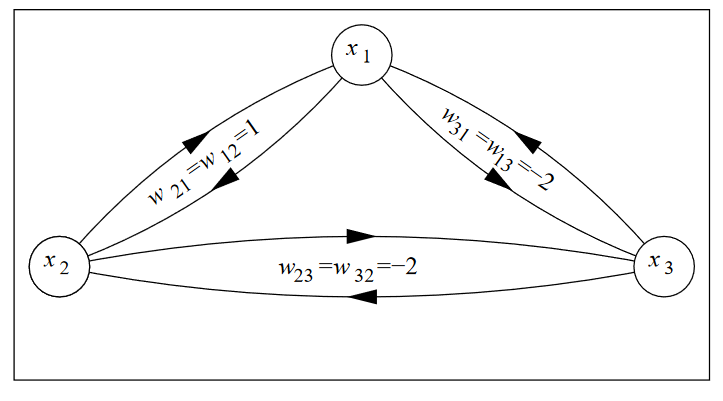
\includegraphics[width=\textwidth]{hopfieldnet}
            \caption{Hopfieldnet met drie neuronen.}
            \label{}
        \end{figure}
        \item De toestand wordt beschreven door de uitvoer van de drie neuronen als een binair getal te beschouwen. 
        \begin{itemize}
            \item Toestand $5 = (+ - +)$ waarbij $x_1$ en $x_3$ als uitvoer 1 hebben en $x_2$ uitvoer -1.
            \item Wat als we in deze toestand $x_2$ aanduiden voor herberekening.
            \item De invoer voor $x_2$ is $1 \cdot 1 - 2 \cdot 1 = -1$, zodat $x_2$ dezelfde uitvoer behoudt, en het net in toestand 5 blijft.
        \end{itemize}
        \item Er kan een transitietabel opgemaakt worden:
        \begin{table}[ht]
            \centering
            \begin{tabular}{| l | c  c  c |}
                \hline
                toestand & \multicolumn{3}{c|}{aangewezen neuron} \\
                \hline
                & $x_1$ & $x_2$ & $x_3$ \\
                \hline
                $0=(---)$ & 4 & 2 & 1 \\
                $1=(--+)$ & 1 & 1 & 1 \\
                $2=(-+-)$ & 6 & 2 & 3 \\
                $3=(-++)$ & 3 & 1 & 3 \\
                $4=(+--)$ & 4 & 6 & 5 \\
                $5=(+-+)$ & 1 & 5 & 5 \\
                $6=(++-)$ & 6 & 6 & 6 \\
                $7=(+++)$ & 3 & 5 & 6 \\
                \hline
            \end{tabular}
        \end{table}
        \item Toestand 6 en 1 zijn stabiel. Elke andere toestand zal ooit in toestand 1 of 6 komen door willekeurig neuronen aan te duiden.
        \begin{figure}[ht]
            \centering
            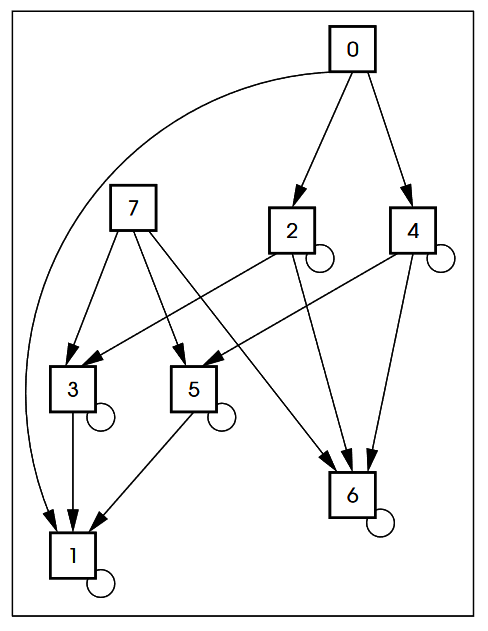
\includegraphics[width=0.5\textwidth]{overgangsdiagram}
            \caption{Overgangsdiagram van het netwerk.}
            \label{}
        \end{figure}
        \item Toestand 6 en 1 komen overeen met de twee patronen die het netwerk heeft opgeslagen. Bij een begintoestand (willekeurig bitpatroon van 3 bits) zal het netwerk evulueren naar één van deze twee toestanden, en wel diegene dat er het best op lijkt.
    \end{itemize}
\end{itemize}
\subsection{Algemene Hopfieldnetten}
\begin{itemize}
    \item Vorig voorbeeld was heel klein, stel nu een groter netwerk, met bijvoorbeeld duizend neuronen ($= 2^{1000}$ toestanden).
    \item De \textbf{energie} van een netwerk met $n$ neuronen wordt gedefinieerd als:
    $$E = -\frac{1}{2}\sum_{i=1}^{n}\sum_{j=1}^{n} \omega_{ij}u_iu_j$$ 
    \begin{itemize}
        \item Het product $u_iu_j$ is altijd gelijk aan $\pm 1$.
        \item Als $w_{ij}$ positief is, dan probeert de verbinding ervoor te zorgen dat $u_i$ en $u_j$ hetzelfde teken krijgen. Hoe groter de waarde $w_{ij}$, hoe meer het resultaat als 'vreemd' beschouwd wordt.
        \item Als $w_{ij}$ negatief is, dan is alles omgekeerd.
    \end{itemize}
    \item De energie van een net is een maat voor hoe vreemd de toestand is van het net.
    \item Duidt een neuron $x_k$ aan voor herberekening. \textbf{Twee} mogelijkheden:
    \begin{enumerate}
        \item De waarde van het neuron blijft hetzelfde zodat de toestand en energie behouden blijft.
        \item De waarde van het neuron verandert. Wat is nu de invloed hiervan op de energie van het netwerk?
        \begin{align*}
          E & = -\frac{1}{2}\sum_{i \neq k}^{n}\sum_{j \neq k}^{n} \omega_{ij}u_iu_j  -\frac{1}{2}\sum_{j} \omega_{kj}u_ku_j   -\frac{1}{2}\sum_{i} \omega_{ik}u_iu_k  \\
            & = -\frac{1}{2}\sum_{i \neq k}^{n}\sum_{j \neq k}^{n} \omega_{ij}u_iu_j -u_k\sum_{i \neq k}w_{ik}u_i
        \end{align*}
        \item De verandering van energieniveau is dan:

    \end{enumerate}
\end{itemize}
\section{Leren bij Hopfieldnetten}
\begin{itemize}
    \item Via de regel van Hebb.
    \item Als we de kans willen vergroten dat een bepaald patroon $U = (u_1, ..., u_n)$ als uitvoer voorkomt, dan moet de energie van dit patroon vermindert worden. 
    \begin{itemize}
        \item Dit komt neer met het veranderen van de gewichten in de richting van de uitvoeren:
        $$w_{ij} \rightarrow w_{ij} + u_iu_j \; \hbox{voor}\; i \neq j$$
        \item De wijziging in energie:
        \begin{align*}
            E_{nieuw}(U) & = -\frac{1}{2}\sum_{i=1}^{n}\sum_{j=1}^{n} (\omega_{ij} + \Delta\omega_{ij})u_iu_j \\
                         & = E_{oud}(U) -\frac{1}{2}\sum_{i=1}^{n}\sum_{j=1}^{n} \Delta\omega_{ij}u_iu_j  \\
                         & = E_{oud}(U) -\frac{1}{2}\sum_{i=1}^{n}\sum_{j=1}^{n} 1 \\
                         & = E_{oud}(U) - \frac{n^2 - n}{2}
        \end{align*}
    \end{itemize}
    \item Voor een ander patroon $V = (v_1, ..., v_n)$ die $k$ bits verschilt van $U$ daalt de energie ook:
    \begin{itemize}
        \item \begin{align*}
            E_{nieuw}(V) & = -\frac{1}{2}\sum_{i=1}^{n}\sum_{j=1}^{n} (\omega_{ij} + \Delta\omega_{ij})v_iv_j \\
                         & = E_{oud}(V) -\frac{1}{2}\sum_{i=1}^{n}\sum_{j=1}^{n} \Delta\omega_{ij}v_iv_j  \\
        \end{align*}
        en
        \begin{figure}[ht]
            \centering
            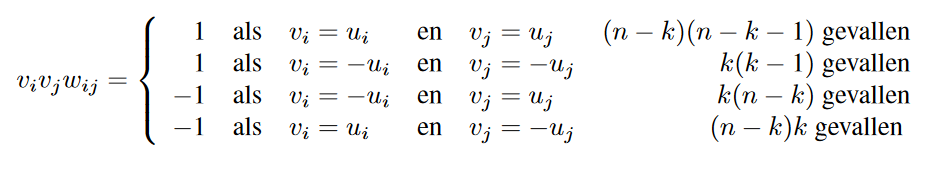
\includegraphics[width=\textwidth]{energy}
        \end{figure}

        dus
        $$E_{nieuw}(V) = E_{oud}(V) - \frac{(2k - n)^2 - n}{2} \\$$
    \end{itemize}

\end{itemize}

\section{Associatieve groepering}
\begin{itemize}
    \item Het komt bijna nooit voor dat dezelfde invoer herhaalde malen voorkomt in het leerproces.
    \item De stabiele eindtoestanden zijn een soort gemiddelde van groepen invoertoestanden die bij elkaar horen.
    \item Hopfieldnetten kunnen dan gebruikt worden om te classificeren zonder supervisie.
    \item Het algoritme:
    \begin{enumerate}
        \item Zet alle gewichten van het associatief geheugen op nul.
        \item Train het associatief geheugen op de gebruikelijke wijze met de gehele verzameling van punten.
        \item Houdt nu de gewichten van het associatief geheugen vast en presenteer weer alle punten. Punten die dezelfde uitvoer geven worden in dezelfde groep gestoken.
    \end{enumerate}
    \item In een andere versie wordt bij stap 3 dezelfde invoer meerdere malen gepresenteerd, maar worden verschillende neuronen gekozen om te herberekenen.
    \begin{itemize}
        \item Een punt dat meerdere uitvoeren heeft, wordt als grenspunt beschouwd.
        \item Als twee groepen meer grenspunten gemeen hebben dan een bepaald opgegeven getal, worden ze samengevoegd.
        \item Dit komt nauw overeen met transitiviteit.
    \end{itemize}
    \item Nog een alternatief: \textbf{winner-takes-all} netwerk:
    \begin{itemize}
        \item Neem $n$ analoge neuronen met uitvoerwaarden tussen $0$ en $1$ zodat het omringende netwerk ervoor zorgt dat de activatie van de neuron een functie is van de waarschijnlijkheid van elk van de alternatieven.
        \item Alle $n$ neuronen zijn nu onderling verbonden met negatieve gewichten.
    \end{itemize}
\end{itemize}

\section{Patroonvervollediging}
\begin{itemize}
    \item 
\end{itemize}
\chapter{Kennisrepresentatie in neurale netten}
\chapter{Een geïntegreerd netwerk}
\begin{itemize}
    \item Kennis van vorige hoofdstukken toepassen op het \textbf{vertaalprobleem}.
\end{itemize}

\section{Het vertaalprobleem}
\begin{itemize}
    \item Dubbelzinngheid in een taal kan zich voordoen op drie niveaus:
    \begin{enumerate}
        \item Een woord kan verschillende betekenissen hebben.
        \item Een woord kan zich in verschillende grammaticale klassen bevinden.
        \item Woorden kunnen gecombineerd worden.
    \end{enumerate}
\end{itemize}

\section{Overzicht van het netwerk}
\begin{itemize}
    \item \begin{enumerate}
        \item De binnenkomende geluiden moeten omgezet worden in een reeks van fonemen.
        \item De fonemenreeksen moeten gesplitst worden in woorden. De woorden voegen we samen in zinnen.
        \item Van deze zinnen moet de grammaticale structuur bepaald worden.
        \item Uit de woorden en de grammaticale structuur moeten we betekenissen halen.
        \item Deze betekenissen moeten omgezet worden in de doeltaal, door de passende grammaticale structuur in de doeltaal te vinden en de juiste woorden daarin in te passen.
        \item De resulterende woordenreeks moet omgezet worden in een fonemenreeks en uitgestuurd worden.
    \end{enumerate}
    \item Een verzameling woorden die instaan voor een begrip (een foneem, een woord, ...) worden clusters genoemd.
    \item Twee belangrijke vormen van clusters:
    \begin{itemize}
        \item Clusters die verband houden met tijdssequentiële data zullen min of meer de vorm aannemen van een \textbf{automaat}.
        \item Clusters die simultane data moeten verwerken gedragen zich als \textbf{associatieve geheugens}.
    \end{itemize}
    \item Het netwerk kan dan in drie eenheden onderscheiden worden:
    \begin{enumerate}
        \item Een woordherkenningseenheid (stap 2).
        \item Een grammaticale eenheid (stap 3).
        \item Een begripseenheid (stap 4).
    \end{enumerate}
    
\end{itemize}

\section{Van foneem naar woord}
\begin{itemize}
    \item Een reeks van fonemen wordt aangeboden.
    \item De tijdsvolgorde is belangrijk.
    \item Er is een aparte herkennende automaat voor elk woord.
    \item Er is een apart detectiecluster voor elk woord die het woord analyseert.
    \item Alle woordautomaten werken parallel en proberen hun woord te herkennen in de invoerstroom.
    \begin{itemize}
        \alert Er zullen veel valse positieven zijn.
    \end{itemize}
    \item Een kort woord kan deel uitmaken van een langer woord.
    \item Detectie van een langer woord moet de detectie van een korter woord onderdrukken.
    \item Er zijn dus terugkoppelingslussen van clusters die een lang woord verstellen naar clusters die een subwoord voorstellen om de subwoorden terug te desactiveren.
\end{itemize}

\section{Van woord naar betekenis}
\begin{itemize}
    \item Het betekenisgebied van het neuraal net bestaat uit verschillende modules die verbonden zijn zoals een Hopfieldnet.
    \item Betekenissen die samen voorkomen zijn verbonden door positieve takken. 
    \item Betekenissen die verbonden zijn met hetzelfde woord zijn verbonden met negatieve takken.
    \item Het is een \textbf{winner-takes-all} netwerk.
\end{itemize}

\section{Grammaticale Analyse}
\begin{itemize}
    \item Via contextvrije grammatica's.
    \begin{align*}
        \langle\textbf{S}\rangle &::= \langle\textbf{WWG}\rangle\langle\textbf{LV}\rangle \\
        \langle\textbf{WWG}\rangle &::= \langle\textbf{SG}\rangle\langle\textbf{WWG}\rangle \\
        \langle\textbf{LV}\rangle &::= \langle\textbf{SG}\rangle \\
        \langle\textbf{SG}\rangle &::= \langle\textbf{LW}\rangle\langle\textbf{SA}\rangle \\
        \langle\textbf{SA}\rangle &::= \langle\textbf{ADJ}\rangle\langle\textbf{SA}\rangle|\langle\textbf{SUB}\rangle \\
        \langle\textbf{LW}\rangle &::=  de\\
        \langle\textbf{ADJ}\rangle &::= blauwe\\
        \langle\textbf{SUB}\rangle &::=  vinvis|garnaal\\
        \langle\textbf{WW}\rangle &::= verorberde\\
    \end{align*}
    \item Voor elke alternatieve substitutie voor een symbool is er een automaat die een lineaire sequentie detecteert bestaande uit de opeenvolging van de activaties van zijn delen.
    
\end{itemize}
\end{document}